% !TeX spellcheck = pl_PL
\section{IEEE-1394 (FireWire)}
Cel projektantów FireWire: stworzenie interfejsu opartego na łączu szeregowym, który mógłby zastąpić równoległy port SCSI. Chodziło o zaprojektowanie bardzo szybkiej magistrali, dogodnej do transferu dużej ilości danych wymienianych z urządzeniami pamięci masowych oraz danych multimedialnych.

\subsection{Możliwości interfejsu IEEE 1394a}
\begin{itemize}
	\item Podłączenie do komputera dużej liczby różnorodnych urządzeń
	\item Wykrywanie włączenia urządzenia do systemu oraz jego odłączenia (\emph{hot plugging})
	\item Automatyczna konfiguracja systemu do komunikacji
	\begin{itemize}
		\item określenie topologii systemu
		\item samoidentyfikacja urządzeń
		\item wyznaczenie szybkości transmisji
		\item konfiguracja urządzeń do komunikacji
	\end{itemize}
	\item Szybka transmisja danych pod kontrolą pakietowego protokołu komunikacyjnego, oparta na transakcjach asynchronicznych i izochronicznych
	\item Rywalizacyjny dostęp urządzeń do łącza pod kontrolą procedury arbitrażowej
	\item Zasilanie urządzenia z systemu
\end{itemize}

\subsection{Topologia i interfejs IEEE 1394a}
Układem umożliwiającym podłączenie komputera opartego na PCI do magistrali szeregowej IEEE 1394 jest most (\emph{Open Host Controller Interface}), który udostępnia zazwyczaj kilka portów IEEE 1394.\\
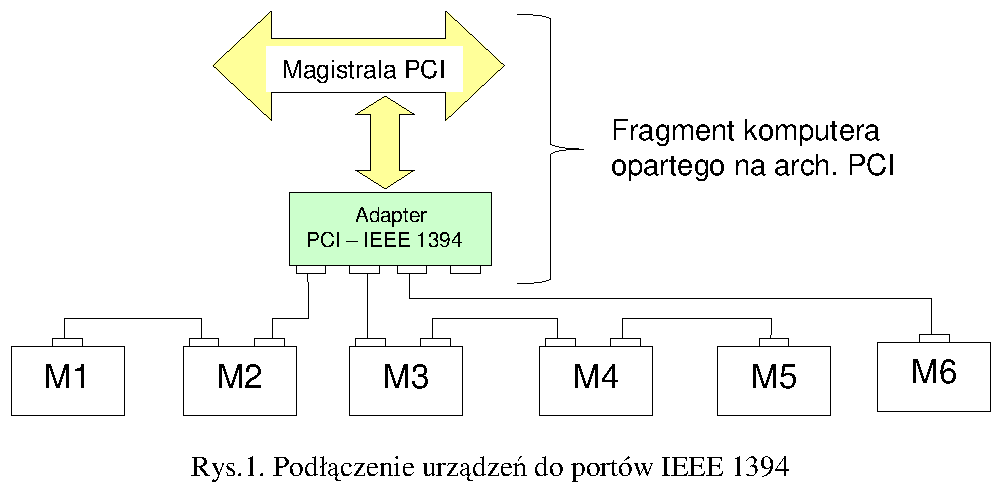
\includegraphics[width=10cm]{./wyklady/FIREWIRE_2_1.pdf}\\
\begin{itemize}
	\item Topologia rozgałęzionej gwiazdy.
	\item Struktura: rozgałęziona magistrala (\emph{daisy chain}).
	\item Poszczególne urządzenia, zwane węzłami, rywalizują ze sobą o dostęp do łącza w celu przesłania porcji danych (pakietu). Pakiety przesyłane są co 125 $\mu s$
	\item \textbf{Urządzenia z jednym portem stanowią zakończenie gałęzi} (liście), urządzenia z wieloma portami umożliwiają rozbudowę gałęzi przez podłączenie kolejnego urządzenia. Liściem może też być urządzenie wieloportowe , w którym wykorzystany jest tylko jeden port.
	\item \textbf{Komunikacja pomiędzy portami oparta jest na zasadzie punkt-punkt} (\emph{point to point}), co dla urządzenia wieloportowego oznacza odbiór i detekcję całego pakietu przez jeden port, a następnie jego resynchronizację do lokalnego zegara i retransmisję do pozostałych portów.
	\item \textbf{System nie posiada hosta}, komunikacja pomiędzy urządzeniami odbywa się bez interwencji stacji nadrzędnej. Ten rodzaj komunikacji określamy jako P2P (\emph{peer to peer})
	\item \textbf{Konfiguracja urządzeń następuje dynamicznie}, bez wykorzystania kontrolera systemu. Interfejsy urządzeń mają wbudowane funkcje konfiguracyjne, które umożliwiają określenie topologii systemu, parametryzację portów urządzeń oraz przekazanie informacji o urządzeniu. Odbywa się po każdym resecie.
\end{itemize}


\subsection{Architektura węzła}
System IEEE 1394 ma topologię rozgałęzionej gwiazdy i oparty jest na transferach bezpośrednich między urządzeniami (brak hosta w systemie).
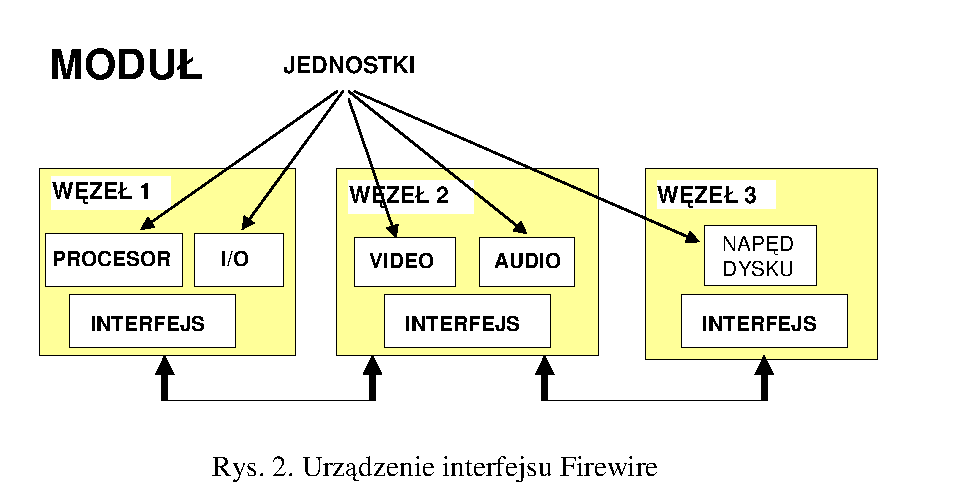
\includegraphics[width=7cm]{./wyklady/FIREWIRE_3_1.pdf}\\
Ważniejsze terminy stosowane w IEEE 1394:
\begin{itemize}
	\item moduł (\emph{module}): fizyczne urządzenie podłączone do magistrali, które może zawierać kilka węzłów
	\item węzeł (\emph{node}): logiczne urządzenie wewnątrz modułu
	\item jednostka (\emph{unit}): element węzła o określonej funkcjonalności (np. procesor, pamięć, I/O)
\end{itemize}

\subsection{Przestrzeń adresowa i jej podział}
Przestrzeń adresowa jest zgodna z IEEE Std 1212-1991 Control and Status Register (CSR) Architecture.\\
\begin{itemize}
	\item Adres zawiera 64 bity podzielone na:
	\begin{itemize}
		\item Numer magistrali (\emph{Bus Number}), 10 najstarszych bitów: Bus 0 do Bus 1023
		\item Numer węzła w ramach magistrali (\emph{Node Number}), 6 bitów: Node 0 do Node 63
		\item Pole adresowe w węźle (\emph{Node Address}), 48 bitów.
	\end{itemize}
	\item Format adresu\\
	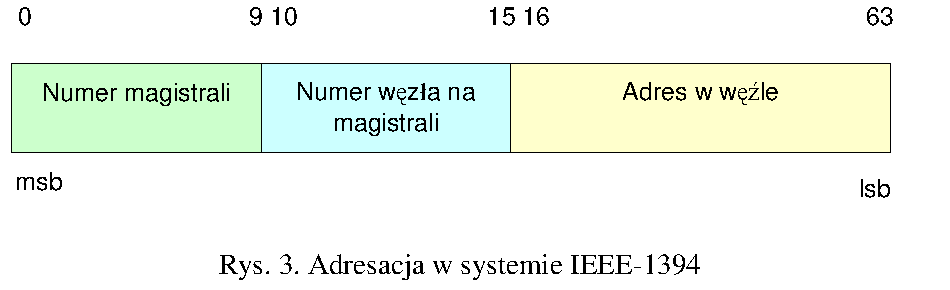
\includegraphics[width=10cm]{./wyklady/FIREWIRE_4_1.pdf}
	\item Podział pamięci węzła\\
	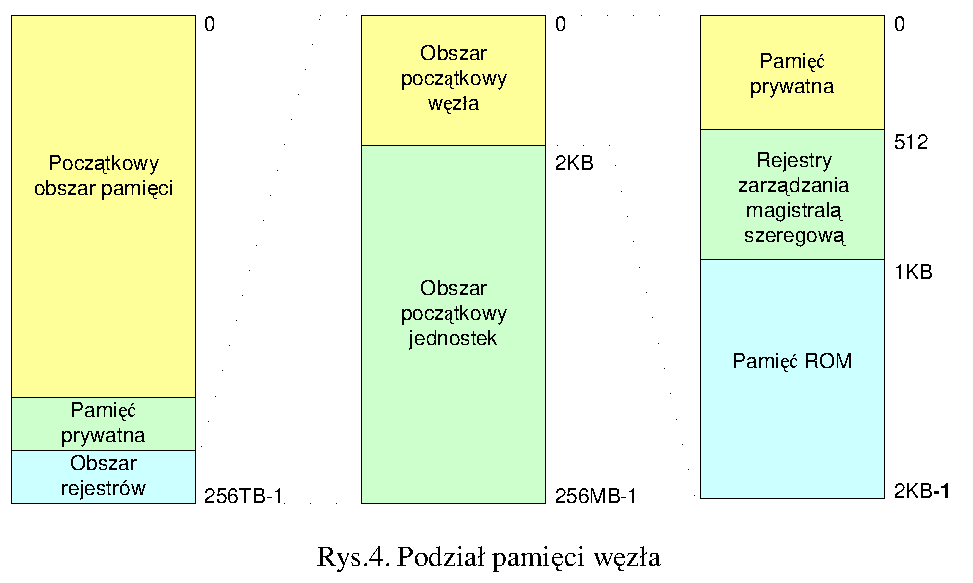
\includegraphics[width=10cm]{./wyklady/FIREWIRE_5_1.pdf}
\end{itemize}


\subsection{Transfery i transakcje}
Zasady komunikacji:
\begin{itemize}
	\item Transfery są żądaniami przesłania danych.
	\item Transfery dzielone są na transakcje (w celu umożliwienia podziału pasma pomiędzy węzłami).
	\item Wyróżnia się transakcje:
	\begin{itemize}
		\item \textbf{Asynchroniczne} - wymagają potwierdzenia (odpowiedzi) i w przypadku błędów są powtarzane. Mogą być wykonywane cyklicznie lub aperiodyczne.
		\item \textbf{Izochroniczne} - nie są potwierdzane. Nie kontroluje się poprawności przesłania danych, a jedynie zapewnia stały rytm ich dostarczania.
	\end{itemize} 
\end{itemize}

	\subsubsection{Transakcje asynchroniczne}
	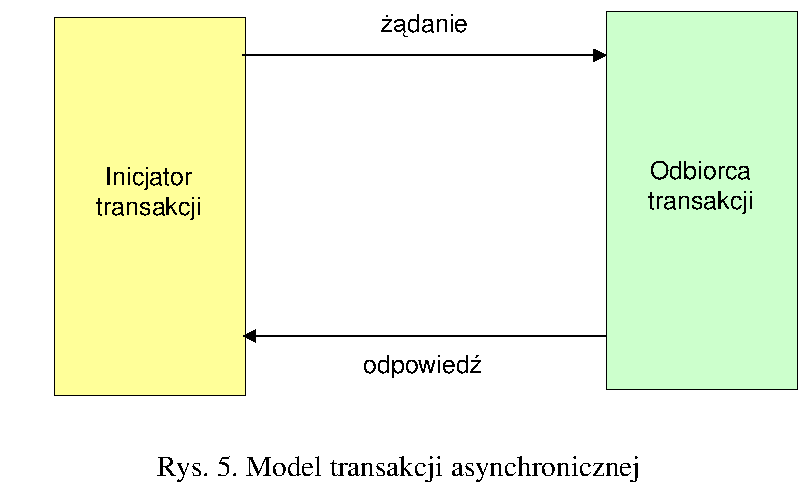
\includegraphics[width=10cm]{./wyklady/FIREWIRE_7_1.pdf}\\
	Rozpoczęcie transakcji nie jest synchronizowane z odbiorcą. Wyróżniono 3 rodzaje transakcji asynchronicznych:
	\begin{itemize}
		\item Odczyt (\emph{read}) - pobranie danych od odbiorcy
		\item Zapis (\emph{write}) - przekazanie danych do odbiorcy
		\item Zamknięcie (\emph{lock}) - odczyt danych, ich modyfikacja i ponowny zapis
	\end{itemize}
	Każdą transakcję rozpoczyna inicjator transakcji (\emph{requester}) i potwierdza odbiorca transakcji (\emph{responder}). Zatem transakcja dzielona jest na dwie części:
	\begin{itemize}
		\item Fazę przekazania żądania (adres, rozkaz i dane)
		\item Fazę przekazania odpowiedzi (przy zapisie - status wykonania, przy odczycie - dane)
	\end{itemize}
	
	\subsubsection{Transakcje izochroniczne}
	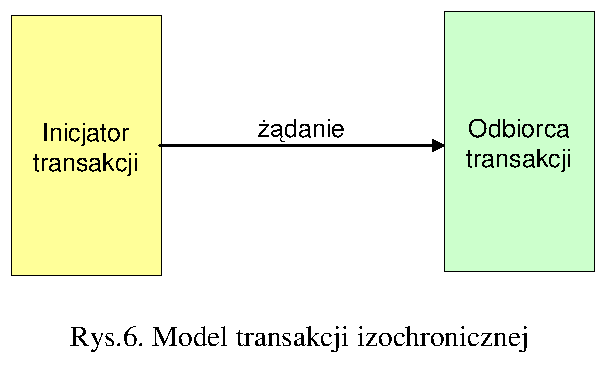
\includegraphics[width=10cm]{./wyklady/FIREWIRE_8_1.pdf}\\
	\begin{itemize}
		\item Transfer izochroniczny zapewnia regularne dostarczanie danych bez sprawdzania ich ważności.
		\item Dane dostarczane są cyklicznie w odstępach 125 $\mu{s}$, bez potwierdzenia ich odbioru przez urządzenie odbierające.
		\item Życie danych izochronicznych jest wyjątkowo krótkie, a ich uszkodzenia nie mają trwałych konsekwencji.
		\item Przykładem mogą być dane cyfrowe reprezentujące dźwięk przesyłane do głośników.
	\end{itemize}

\subsection{Konfiguracja urządzeń do komunikacji, współdzielenie magistrali}
\subsubsection{Konfiguracja}
Po każdym włączeniu zasilania lub zmianie węzłów w systemie (dołączenie lub odłączenie urządzenia) następuje automatyczna konfiguracja magistrali, której rezultatem jest przygotowanie węzłów do działania.\\
Po przeprowadzeniu konfiguracji węzły mogą rywalizować o dostęp do magistrali (arbitraż), a po jego uzyskaniu przekazywać dane.
\subsubsection{Współdzielenie magistrali}
Transakcje asynchroniczne i izochroniczne współdzielą magistralę, ponieważ zarządzanie magistralą „stara się” umożliwić jednoczesne (quasi) jej wykorzystanie przez różne transfery.\\
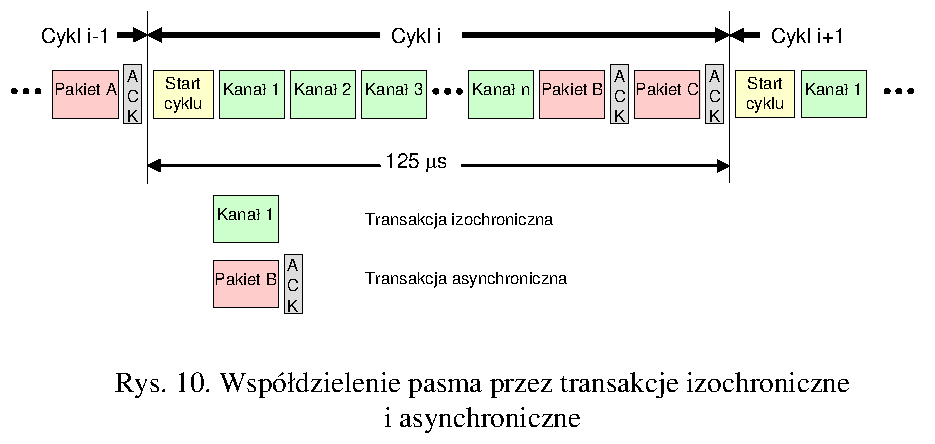
\includegraphics[width=10cm]{./wyklady/FIREWIRE_13_1.pdf}\\

\subsection{Model komunikacyjny}
Podstawowe funkcje warstw protokołu komunikacyjnego:
\begin{itemize}
	\item \textbf{Warstwa zarządzania magistralą} - konfiguracja i zarządzanie węzłem
	\item \textbf{Warstwa transakcji} - świadczy usługi dla transferów asynchronicznych realizując protokół żądanie-odpowiedź określony przez architekturę CSR. Wspiera 3 rodzaje operacji: odczyt, zapis i zamknięcie.
	\item \textbf{Warstwa połączeniowa} - wykonuje transakcję generując sekwencję pakietów w stacji nadrzędnej i odbierającej.
	\item \textbf{Warstwa fizyczna} - zapewnia elektryczny i mechaniczny interfejs szeregowej magistrali oraz wykonuje arbitraż w celu udostępnienia łącza tylko jednemu nadawcy (ochrona przed kolizją).
\end{itemize}
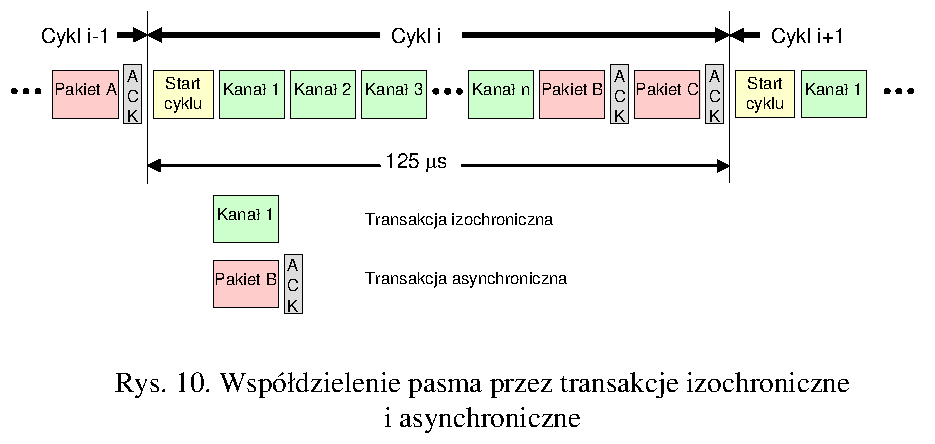
\includegraphics[width=10cm]{./wyklady/FIREWIRE_13_1.pdf}

	\subsubsection{Warstwa zarządzania magistralą}
	Zarządzanie magistralą obejmuje automatyczną konfiguracje węzła do komunikacji oraz, opcjonalnie, zarządzanie dystrybucją zasilania.\\
	Zarządzenia globalne obejmuje:
	\begin{itemize}
		\item przypisanie numeru kanału i pasma transferom izochronicznym
		\item kontrolę odstępów czasowych wykonywania transakcji izochronicznych
		\item kontrolę zasilania węzłów
		\item "dostrajanie" magistrali w celu polepszenia wydajności
		\item świadczenie usług dla innych węzłów, jak np. ustawienie maksymalnej szybkości transmisji pomiędzy węzłami
	\end{itemize}
	
	\subsubsection{Warstwa transakcji}
	Świadczy usługi dla transferów asynchronicznych, które umożliwiają:
	\begin{itemize}
		\item wykonanie odczytu z urządzenia (\emph{read})
		\item wykonanie zapisu danych do urządzenia (\emph{write})
		\item wykonanie modyfikacji danych w urządzeniu (\emph{lock})
	\end{itemize}
	Inicjatorem transakcji jest warstwa aplikacji, która zleca jej wykonanie warstwie transakcji. Model wykonania transkcji wyróżnia inicjatora (\emph{requester}) oraz odbiorcę (\emph{responder}), a także dzieli transakcję na dwie operacje: wysłanie żądania i odebranie odpowiedzi.
	Transakcja asynchroniczna z potwierdzeniem żądania i odpowiedzi (pakietów).\\
	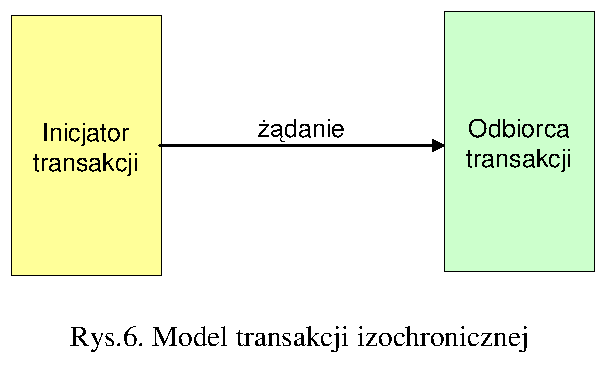
\includegraphics[width=10cm]{./wyklady/FIREWIRE_8_1.pdf}
	
	\subsubsection{Warstwa połączeniowa}
	Oparta na modelu żądanie-odpowiedź.
	\begin{itemize}
		\item Dla transferów asynchronicznych
		\begin{itemize}
			\item Warstwa połączeniowa węzła inicjującego transakcję dokonuje translacji żądania wykonania transakcji na pakiety przekazywane do warstwy fizycznej.
			\item Warstwa połączeniowa węzła odbierającego dokonuje operacji odwrotnej - przekształca odebrane z warstwy fizycznej pakiety i przekazuje je do warstwy transakcji.
		\end{itemize}
		\item Dla transferów izochronicznych jest podobnie, tylko żądanie wykonania transakcji (w węźle inicjującym) przekazywane jest do warstwy połączeniowej bezpośrednio przez sterownik programowy, a pakiety w warstwie połączeniowej u odbiorcy przekazywane są bezpośrednio do sterownika programowego.
	\end{itemize}
	Warstwa połączeniowa wykonuje również transakcje specjalne:
	\begin{itemize}
		\item Transakcja dzielona (\emph{Split Transaction}) - rozpoczęcie kolejnej transakcji przed zakończeniem poprzedniej. Pozwala na lepsze wykorzystanie magistrali i niezablokowanie jej.\\
		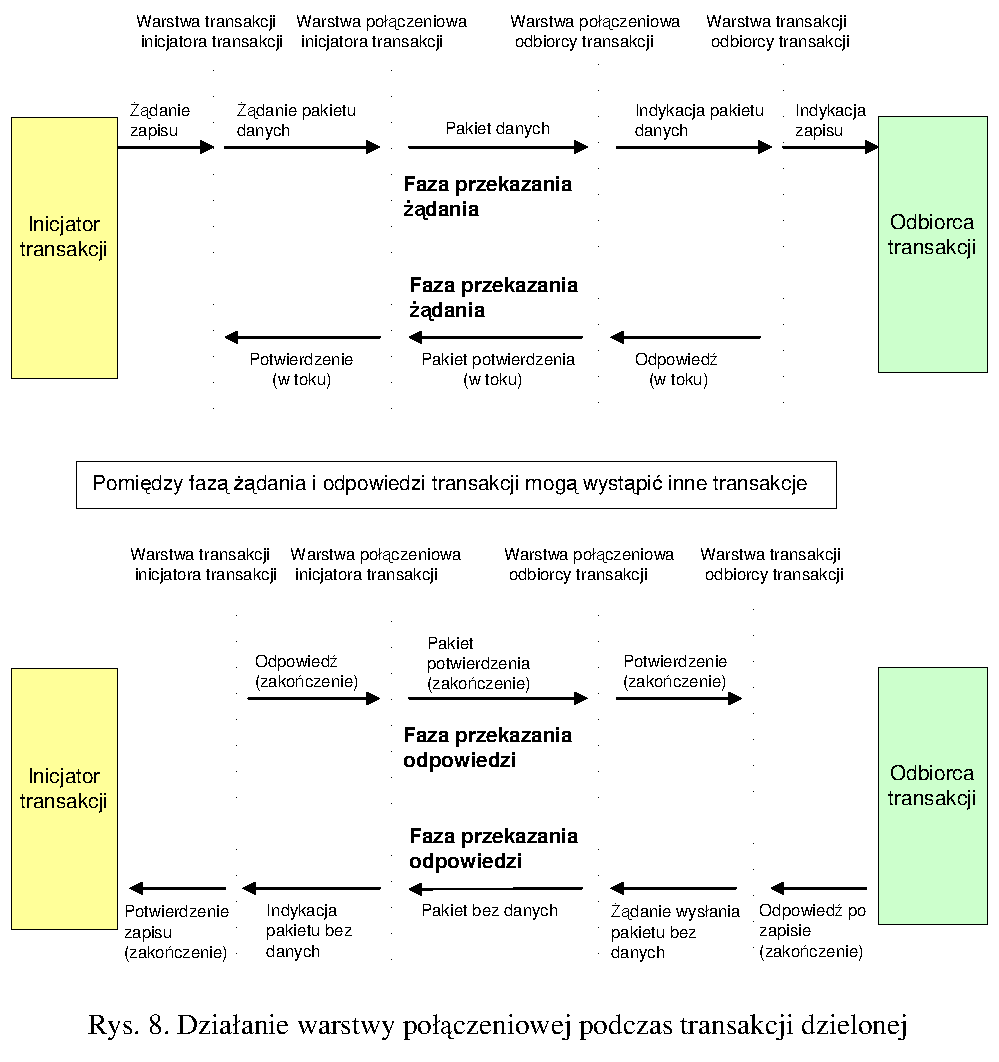
\includegraphics[width=10cm]{./wyklady/FIREWIRE_10_1.pdf}
		\item Transakcja dołączana (concatetated transaction) - umożliwia wykorzystanie magistrali przez inne węzły podczas gdy odbiorca transakcji opóźnia odesłanie odpowiedzi. Kiedy odpowiedź będzie już gotowa, odbiorca musi na drodze arbitrażu uzyskac dostęp do łącza (co wydłuża transakcję).\\
		Jeżeli jednak odbiorca jest zdolny do szybkiego udzielania odpowiedzi, może ją dołączyć do pakietu potwierdzenia wysyłanego w fazie przekazania żądania), co sprawia, że odbiorca transakcji nie musi rywalizować o dostęp do magistrali. Jest to transakcja dołączana.
		\item Transakcja zespolona (Unified Transaction) - to samo co transakcja dołączana, tylko ograniczona do operacji zapisu. Umożliwia włączenie odpowiedzi do potwierdzenia zamykającego fazę przekazania żądania. Sprawia to, że faza przekazania odpowiedzi jest niepotrzebna.\\
		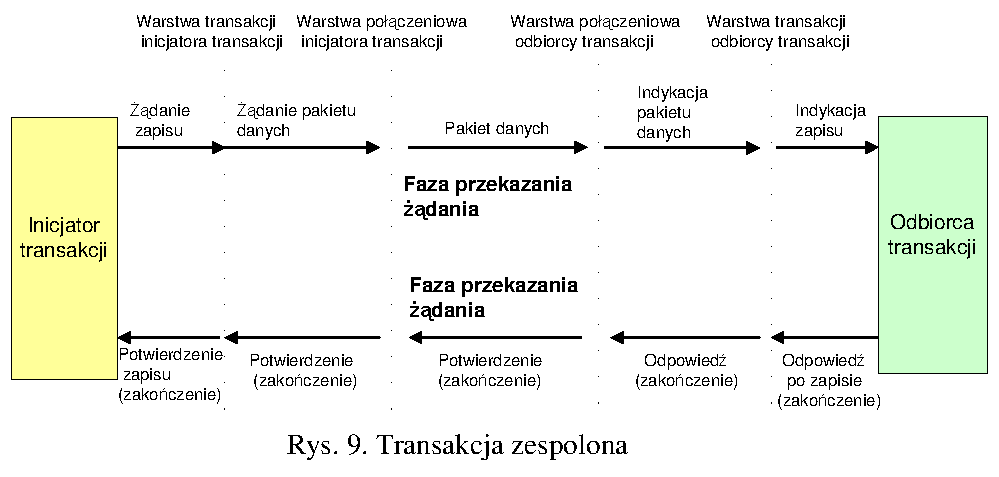
\includegraphics[width=10cm]{./wyklady/FIREWIRE_11_1.pdf}
	\end{itemize}
	\subsubsection{Warstwa fizyczna}
	Prosty węzeł systemu IEEE 1394 z dwoma portami i liniami sygnałowymi magistrali.\\
	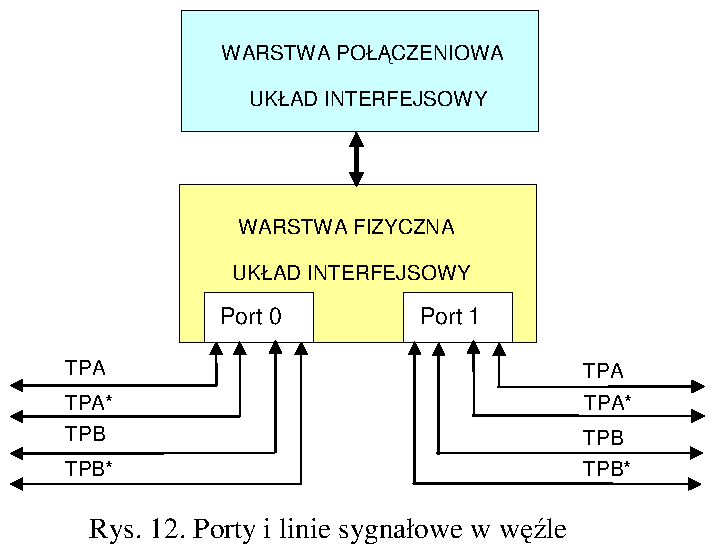
\includegraphics[width=10cm]{./wyklady/FIREWIRE_15_1.pdf}\\\\
	Podstawowe operacje realizowane na liniach sygnałowych:
	\begin{itemize}
		\item \textbf{Konfiguracja} - wykonywana po włączeniu zasilania oraz dołączeniu urządzania do magistrali bądź odłączenia z niej. Przygotowuje (wszystkie) węzły systemu do wymiany informacji.
		\item \textbf{Arbitraż} - konieczny jeżeli w toku jest kilka transakcji realizowanych przez różne węzły. Rywalizują one o dostęp do magistrali, a konflikt rozstrzyga procedura arbitrażowa. Konieczny przed przekazywaniem pakietu żądania i odpowiedzi, niekonieczny dla pakietu potwierdzenia.\\
		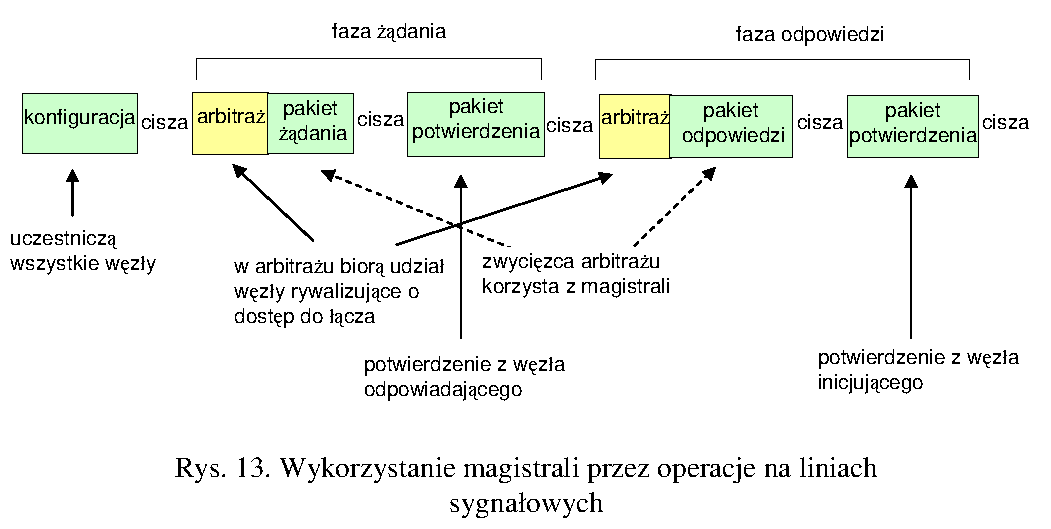
\includegraphics[width=10cm]{./wyklady/FIREWIRE_15_2.pdf}
		\item Przesył danych - prawo tego urządzenia, kto wywalczyło dostęp do magistrali. Dane kodowane są w zapisie NRZ (\emph{Non Return to Zero}).
	\end{itemize}
	\textbf{Szybkość transmisji}\\
	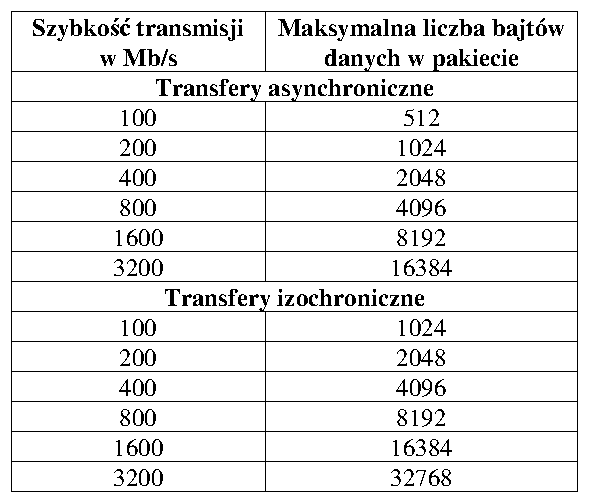
\includegraphics[width=7cm]{./wyklady/FIREWIRE_16_1.pdf}\\
	Minimum musi być spełnione! Szybkość transmisji może być większa, ale nie musi.
	\\\\
	\textbf{Transakcja asynchroniczna}\\
	Jest to transakcja odczytu pomiędzy węzłami A i B (aplikacja w węźle B udostępnia dane tej w A).\\
	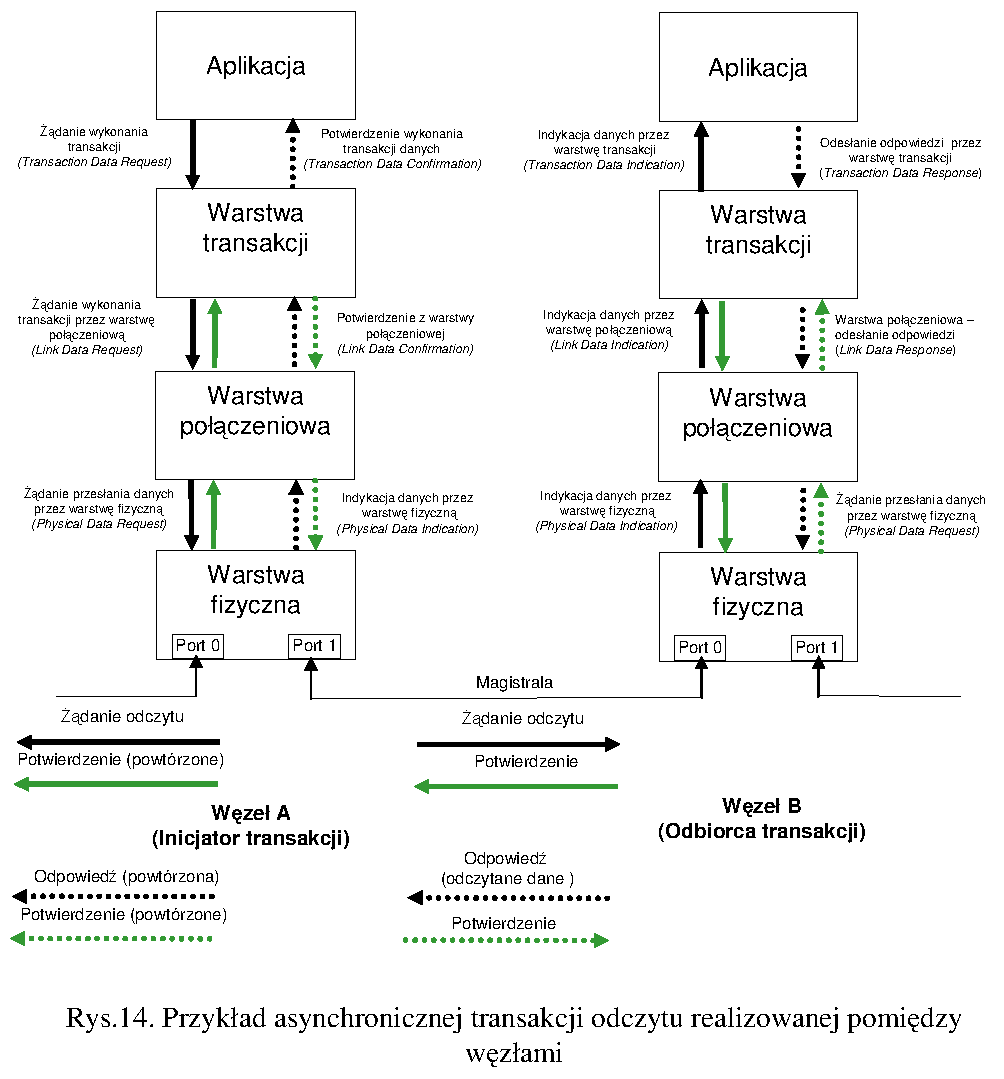
\includegraphics[width=7cm]{./wyklady/FIREWIRE_17_1.pdf}
	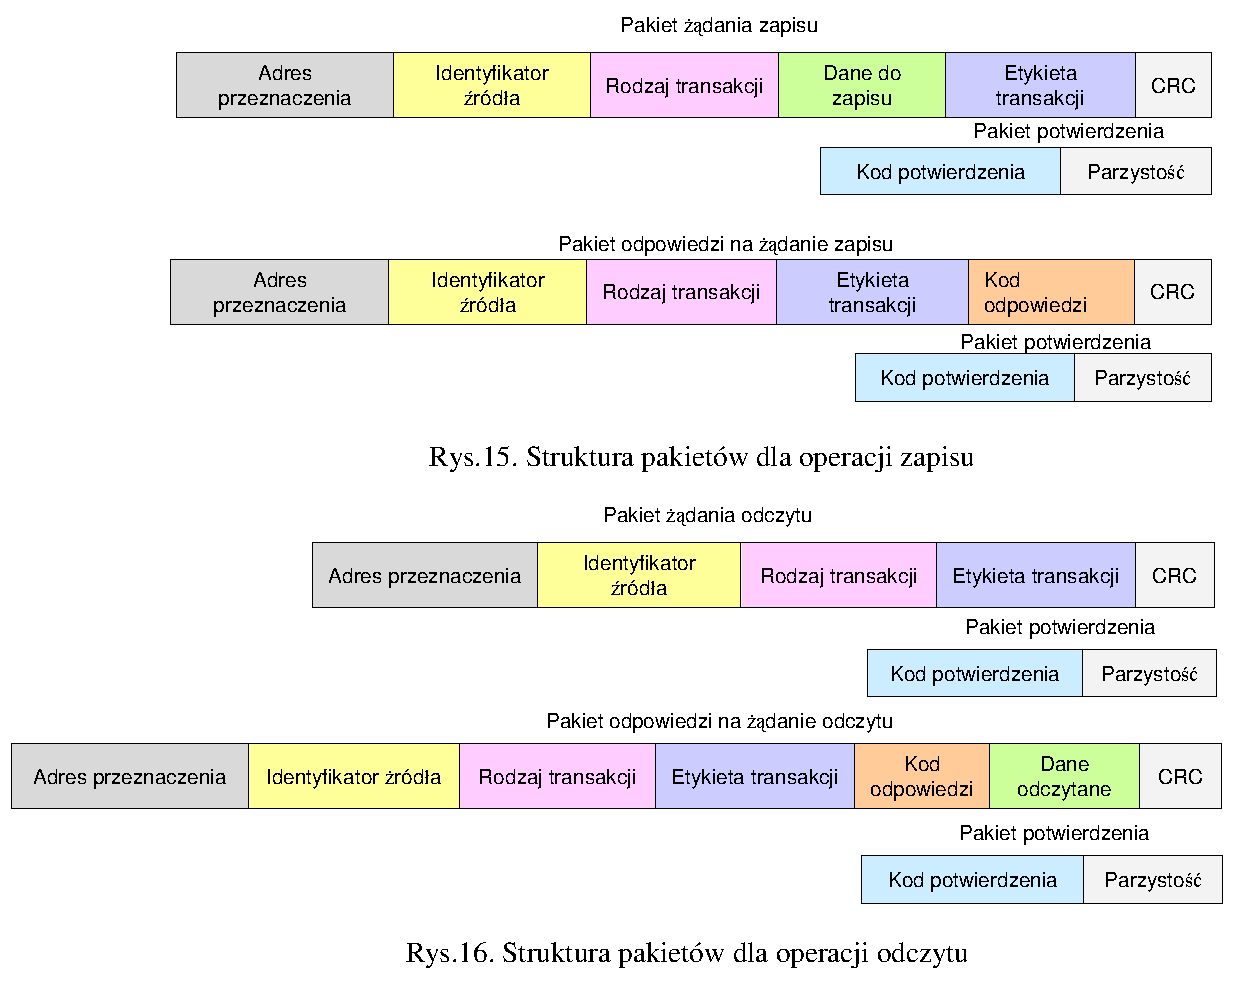
\includegraphics[width=7cm]{./wyklady/FIREWIRE_18_1.pdf}\\\\
	\textbf{Transakcja izochroniczna}\\
	Wykonywane pomiędzy aplikacją, a warstwą połączeniową, z pominięciem warstwy transakcji. Brak potwierdzania pakietów. Często mają charakter rozgłoszenia.\\
	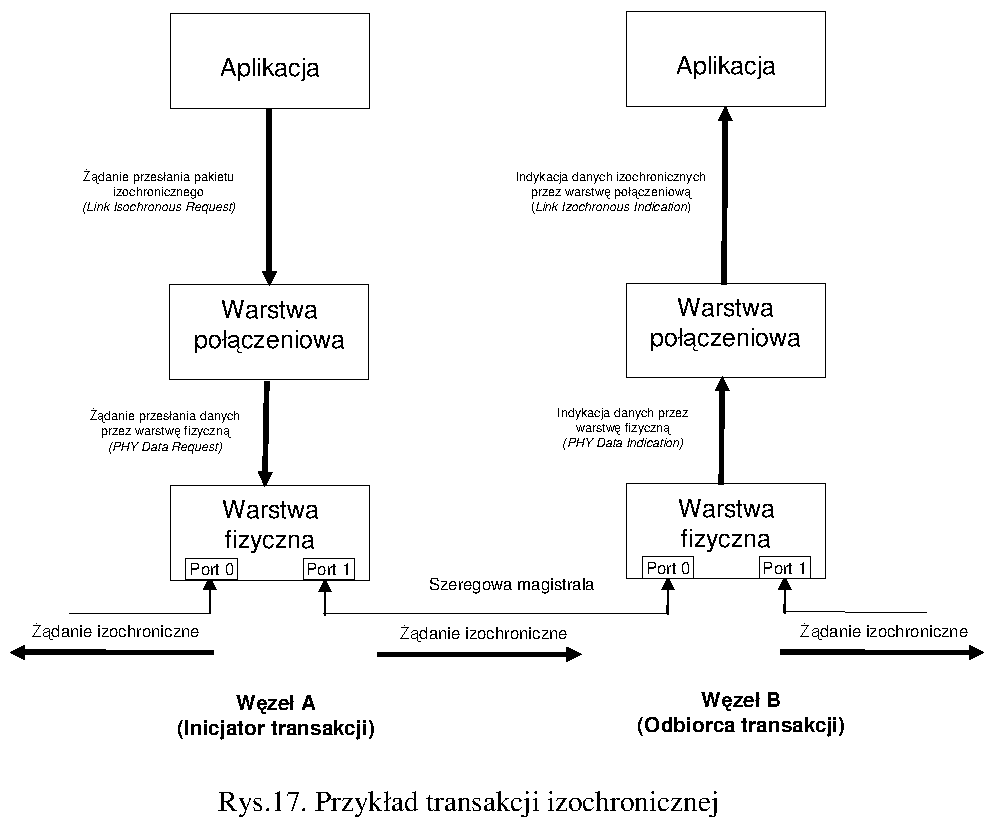
\includegraphics[width=7cm]{./wyklady/FIREWIRE_19_1.pdf}\\\\
	Pakiety w transakcjach izochronicznych.\\
	Transakcje izochroniczne są jednokierunkowe i ograniczają się tylko do przekazania danych przez węzeł inicjujący transakcję. Odbiorca nie odsyła żadnej odpowiedzi. Znaczenie pól typowej transakcji izochronicznej:
	\begin{itemize}
		\item Numer kanału (Channel Number) – węzły uczestniczące w transakcji izochronicznej wykorzystują numer kanału jako adres,
		\item Rodzaj transakcji(Transaction Type) – definiuje rodzaj przesyłanego pakietu jako „izochroniczny”.
		\item Dane (Data) – przekazywane dane,
		\item CRC – suma kontrolna.
	\end{itemize}
	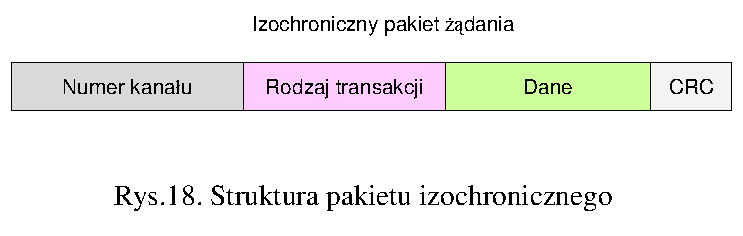
\includegraphics[width=9cm]{./wyklady/FIREWIRE_20_1.pdf}
	
	
\subsection{Interfejs fizyczny}
Obejmuje złącza, okablowanie  oraz układ elektryczny, spełnia funkcje takie jak:
\begin{itemize}
	\item nadawanie i odbiór sygnałów
	\item generacja i rozpoznawanie stanów interfejsu
	\item sygnalizacja maksymalnej szybkości transmisji akceptowanej przez dany port
\end{itemize}
W skład interfejsu fizycznego wchodzi również układ dystrybucji zasilania (umożliwia zasilanie węzłów, które nie mają własnych jednostek zasilających).\\
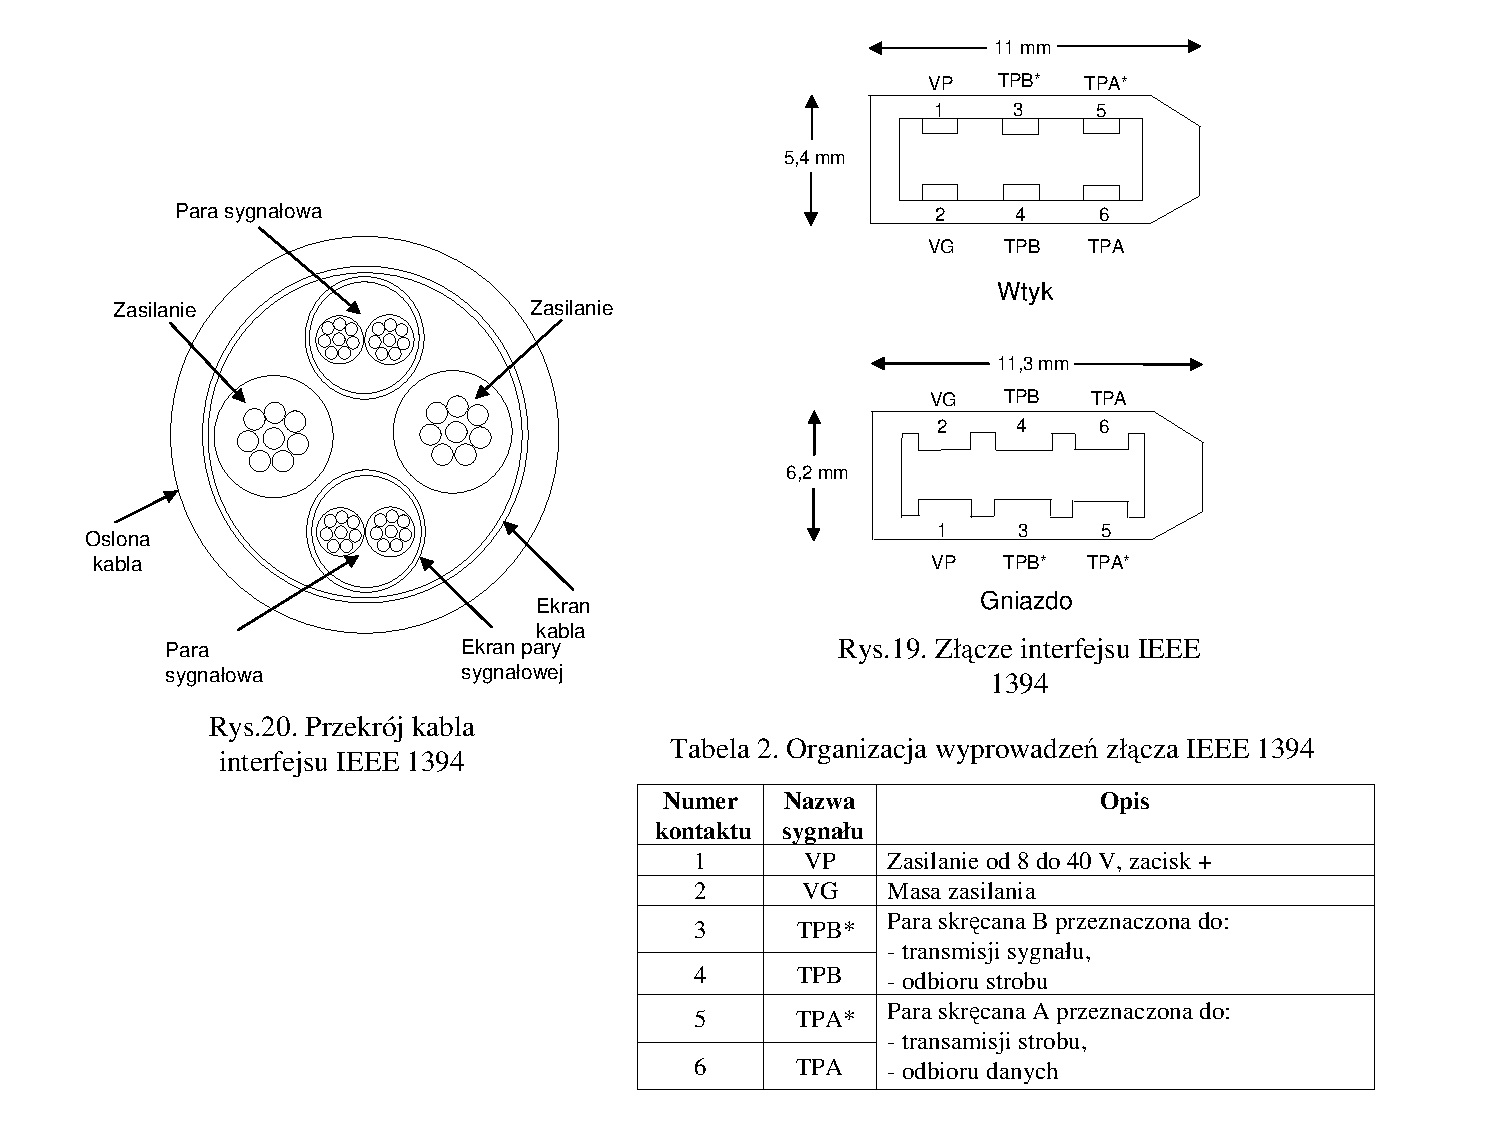
\includegraphics[width=9cm]{./wyklady/FIREWIRE_21_1.pdf}\\\\
W złączach zaciski zasilania są trochę wysunięte do przodu, co sprawia, że przy wdzióbywaniu najpierw doprowadzane jest zasilanie, a potem pojawia się kontakt na liniach sygnałowych.


\subsection{Interfejs sygnałowy}
Interfejs sygnałowy jest bardzo rozbudowy, ponieważ służy nie tylko do transmisji i odbioru danych, ale także do realizacji funkcji arbitrażowych.\\
\textbf{Sygnał różnicowy} - napięcie pomiędzy TPA/TPB, a TPA*/TPB*.\\
\begin{itemize}
	\item TPA/TPA* - linia do przekazywania Strobe
	\item TPB/TBP* - linia do transmisji danych
\end{itemize}
Kodowanie bitów odbywa się w zapisach RZ (\emph{Return to Zero}) oraz NRZ (\emph{Non Return to Zero}).\\
Poniżej odtworzony zegar w interfejsie IEEE 1394. Zegar w węźle odbierającym jest przesunięty czasowo w stosunku do sygnałów Data i Strobe na wyjściu węzła nadającego, ponieważ sygnały ulegają opóźnieniom podczas transmisji w kablu.\\
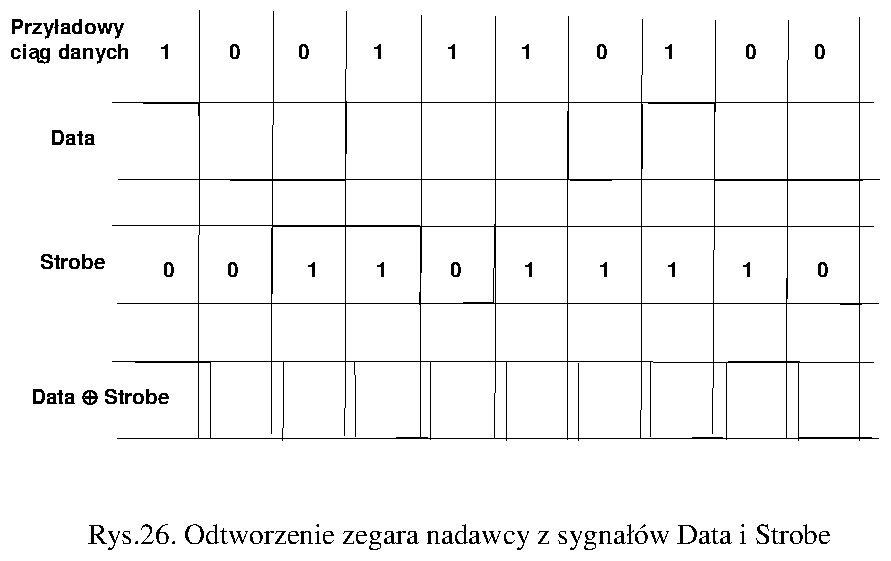
\includegraphics[width=9cm]{./wyklady/FIREWIRE_28_1.pdf}\\\\
Zasada: w wyniku sumowania XOR bitów Data i Strobe uzyskać ciąg występujących na przemian 0 i 1, czemu odpowiada sygnał impulsowy o współczynniku wypełnienia 0.5 i półokresie odpowiadającym bitowej szybkości transmisji.\\\\
\textbf{Sygnalizacja arbitrażu} obejmuje 5 funkcji:
\begin{itemize}
	\item reset magistrali
	\item identyfikacja drzewa
	\item identyfikacja węzła
	\item normalny arbitraż
	\item pakiety startowy i końcowy
	\item sterowanie stanem portu (od wersji 1394a)
\end{itemize}
textbf{Przerwy czasowe} - pomiędzy poszczególnymi fazami składającymi się na transakcję potrzebne są przerwy czasowe podczas których magistrala pozostaje w stanie jałowym.\\
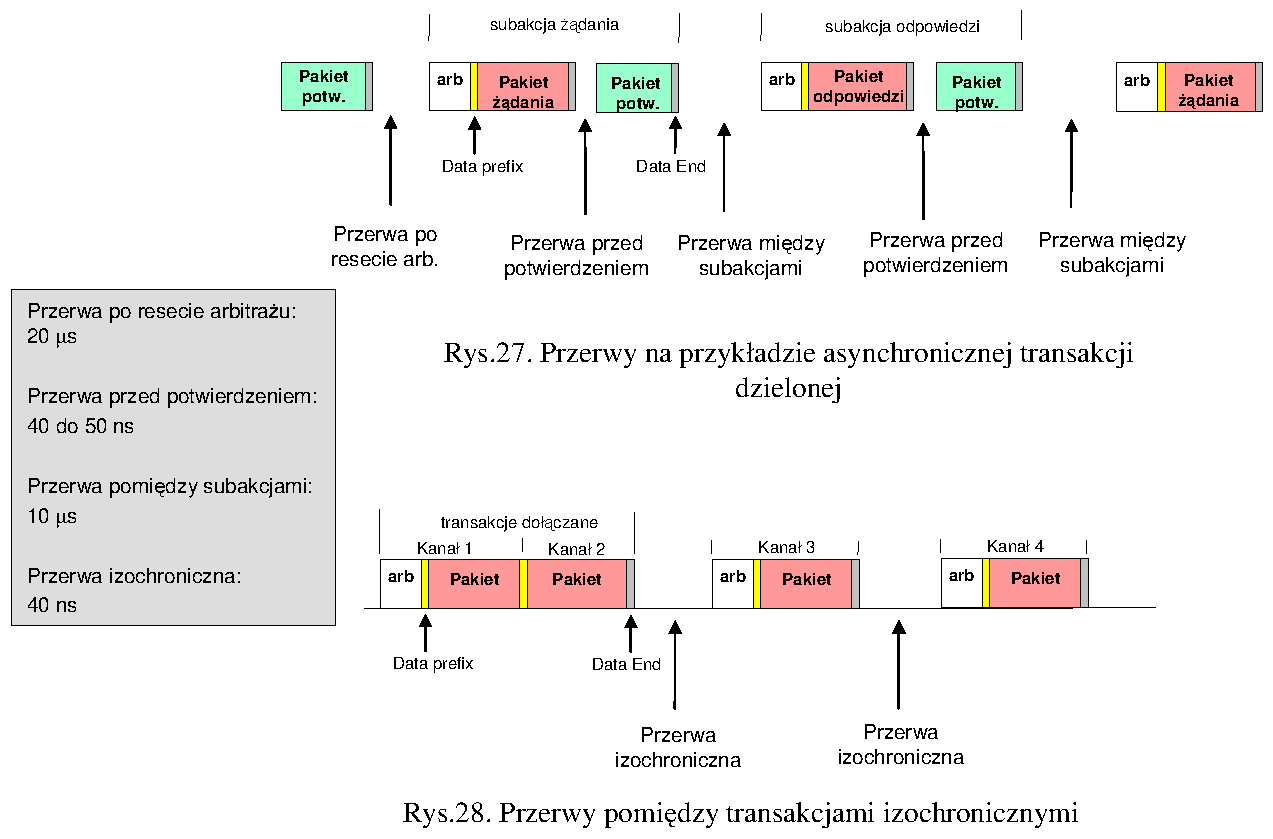
\includegraphics[width=9cm]{./wyklady/FIREWIRE_29_1.pdf}\\
\begin{itemize}
	\item \textbf{Przerwa przed potwierdzeniem} - czas pomiędzy zakończeniem asynchronicznego pakietu (żądania lub odpowiedzi), a rozpoczęciem transmisji pakietu potwierdzenia.
	\item \textbf{Przerwa izochroniczna} - przeznaczona dla kanałów izochronicznych, zapewnia stan jałowy przed rozpoczęciem arbitrażu węzłów izochronicznych. krótsza niż przerwa dla kanałów asynchronicznych.
	\item \textbf{przerwa pomiędzy subakcjami} - dla kanałów asynchronicznych, zapewnia stan jałowy przed rozpoczęciem arbitrażu węzłów izochronicznych. Nie występuje między żądaniem a odpowiedzią w przypadku transmisji dołączanej.
	\item \textbf{Przerwa po resecie arbitrażu} - poprzedza "Interwał równych szans".
\end{itemize}

\subsection{Detekcja szybkości transmisji}
Ze względu na szybkość transmisji wyróżnia się 3 rodzaje portów:
\begin{itemize}
	\item transmisja tylko z szybkością podstawową S100
	\item transmisja z szybkością S100 lub S200
	\item transmisja z szybkością S100, S200 lub S400
\end{itemize}
Gdzie
\begin{itemize}
	\item S100 = 98.304 Mb/s
	\item S200 = 196.608 Mb/s
	\item S400 = 393.216 Mb/s
\end{itemize}
Tylko szybkość S100 jest obligatoryjna dla węzłów. Pozostałe dwa mogą, ale muszą być dostępne. Jeżeli jednak są, to wymagane są układy sygnalizacji szybkości transmisji.\\
Informacja o możliwych szybkościach transmisji każdego węzła przekazywana jest do innych węzłów rezydujących na magistrali podczas konfiguracji (w szczególności informacja o maksymalnej szybkości transmisji przekazywana jest do węzła podłączonego do tego samego segmentu kabla).\\
Zasadą jest nieprzekazywanie przez węzeł pakietów otrzymywanych z daną szybkością do podłączonych do niego węzłów o mniejszej szybkości.\\
Węzeł może mieć kilka portów, przez niektóre porty może być połączony z węzłami o szybkości większej od podstawowej, a przez inne z węzłami o szybkości podstawowej (zatem możliwa jest sytuacja, gdy węzeł odbiera pakiet z szybkością większą od podstawowej, przekazywany przez inny "szybki" węzeł, ale nie będzie go mógł przekazać do węzłów "wolniejszych").\\
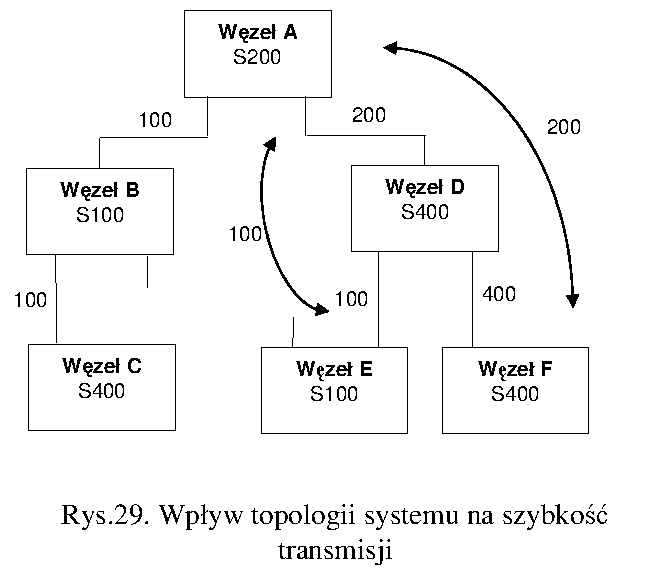
\includegraphics[width=9cm]{./wyklady/FIREWIRE_31_1.pdf}


\subsection{Dystrybucja zasilania}
Węzły w systemie IEEE 1394 mogą być źródłem zasilania dla innych węzłów, korzystać z zasilania przez inne węzły lub też wykorzystywać zasilanie własne bez udostępniania go innym węzłom.\\
\subsubsection{Klasa zasilania}
Węzły wysyłają informację o zasilaniu w ramach pakietu „samoidentyfikacji” (\emph{self-ID}) podczas procesu konfiguracyjnego. Informacja ta przedstawia zapotrzebowania na zasilanie lub możliwość dostarczenia zasilania.\\
Informacje o zasilaniu przekazywane są na 3 bitowym polu \textbf{pwr} w pakiecie self-ID.\\
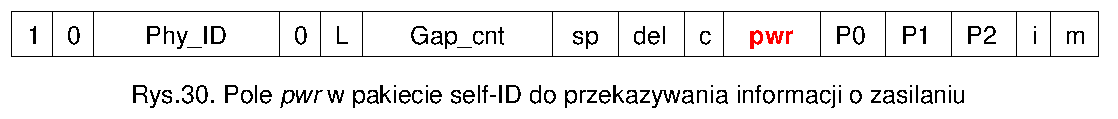
\includegraphics[width=9cm]{./wyklady/FIREWIRE_32_1.pdf}
\subsubsection{Dystrybucja zasilania}
Jeden lub kilka węzłów może jednocześnie być źródłem zasilania. Ponieważ napięcia zasilania udostępniane przez węzły mogą się różnić konieczna jest dioda zapobiegająca przepływowi prądu zasilania do węzła o mniejszym napięciu.\\
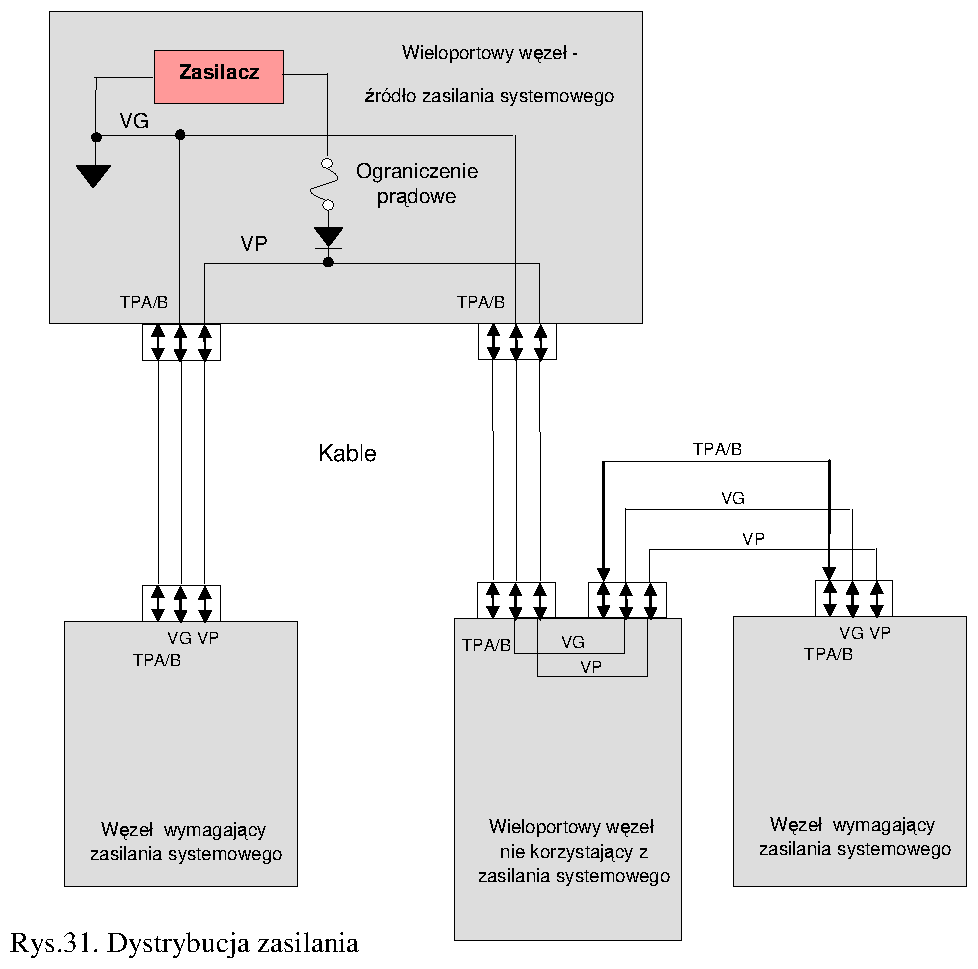
\includegraphics[width=9cm]{./wyklady/FIREWIRE_33_1.pdf}


\subsection{Arbitraż}
W FireWire węzły rywalizują o prawo do nadawania w ramach arbitrażu. Arbitraż realizowany jest w okresach przerw w transmisji (\emph{gaps}) i polega na:
\begin{itemize}
	\item Zagwarantowaniu pasma dla kanałów izochronicznych,
	\item Równoprawnej rywalizacji w przypadku kanałów asynchronicznych.
\end{itemize}
Arbitraż rozpoczyna się po rozpoznania przez węzeł okresu jałowego magistrali, co oznacza koniec poprzedniej transmisji. Czasy trwania jałowych stanów magistrali są różne dla transakcji izochronicznych i asynchronicznych i wynoszą:
\begin{itemize}
	\item Przerwa po resecie arbitrażu: 20 $\mu{s}$
	\item Przerwa pomiędzy subakcjami: 10 $\mu{s}$
	\item Przerwa przed potwierdzeniem: 40 ns
	\item Przerwa izochroniczna - od 40 ns (min) do 50 ns (max),
	\item Przerwa pomiędzy subakcjami transakcji asynchronicznej i przerwa przed potwierdzeniem mogą być „regulowane” (aby arbitraż rozpoczynał się jak najszybciej).
\end{itemize}
Sposób sygnalizowania arbitrażu (protokół sygnalizacji arbitrażu) jest taki sam dla transakcji asynchronicznych i izochronicznych.
\subsubsection{Rodzaje arbitrażu}
Typ pakietu, który jest przygotowany do transmisji, determinuje rodzaj żądania wykorzystywanego przez warstwę połączeniową. Są 4 rodzaje:
\begin{itemize}
	\item  arbitraż oparty na równej szansie dostępu do łącza (\emph{fair arbitration service}) stosowany przy transmisji pakietu asynchronicznego
	\item  arbitraż uwzględniający priorytety (\emph{proirity arbitration service}) stosowany przy transmisji pakietu cycle strat lub pakietu asynchronicznego o wyższym priorytecie
	\item  arbitraż natychmiastowy (\emph{immediate arbitration service}) stosowany przy transmisji pakietu potwierdzenia
	\item  arbitraż izochroniczny (\emph{isochronous arbitration service}) stosowany przy transmisji pakietu izochronicznego
\end{itemize}
\subsubsection{Przykładu arbitrażu}
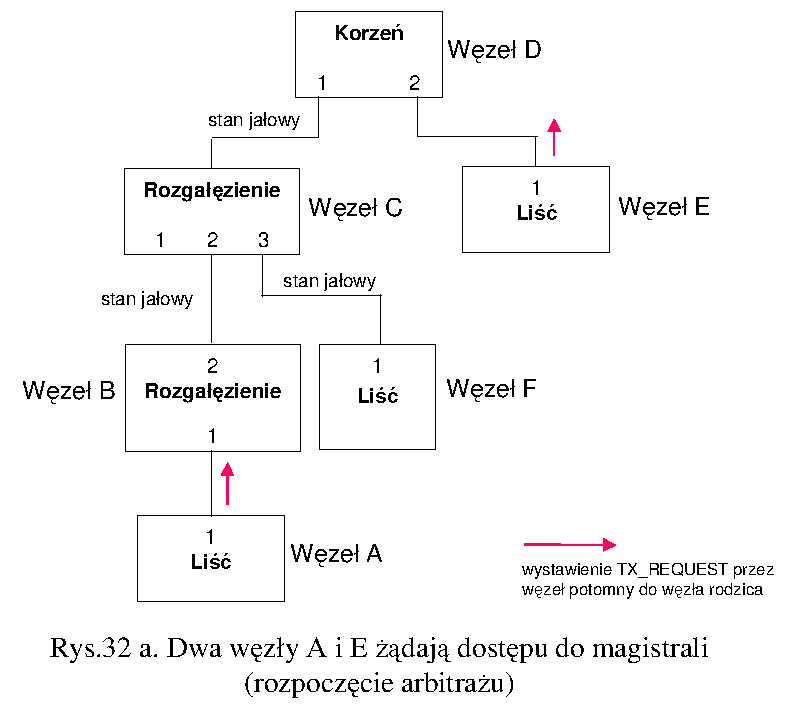
\includegraphics[width=9cm]{./wyklady/FIREWIRE_36_1.pdf}\\\\
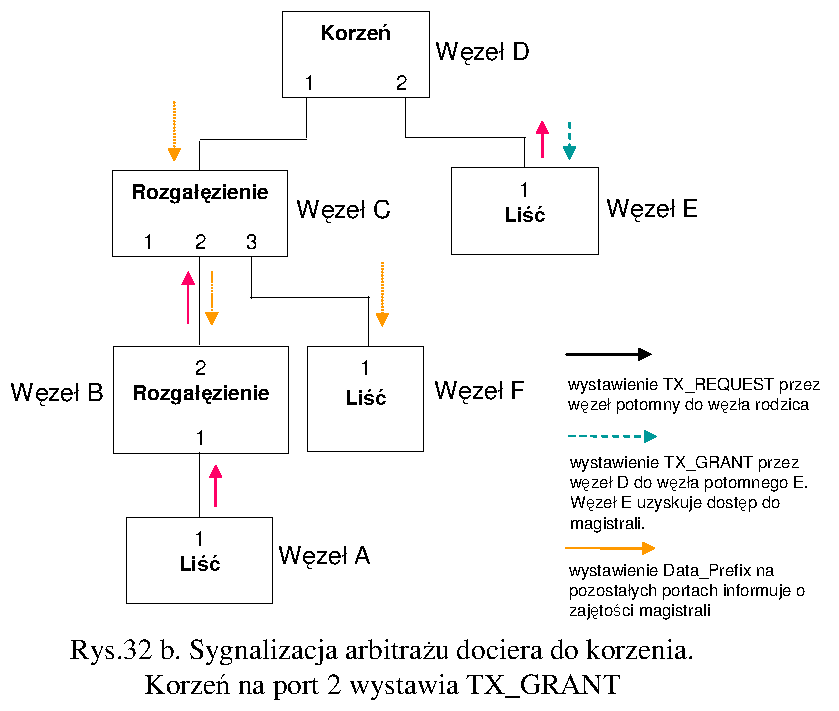
\includegraphics[width=9cm]{./wyklady/FIREWIRE_37_1.pdf}\\\\
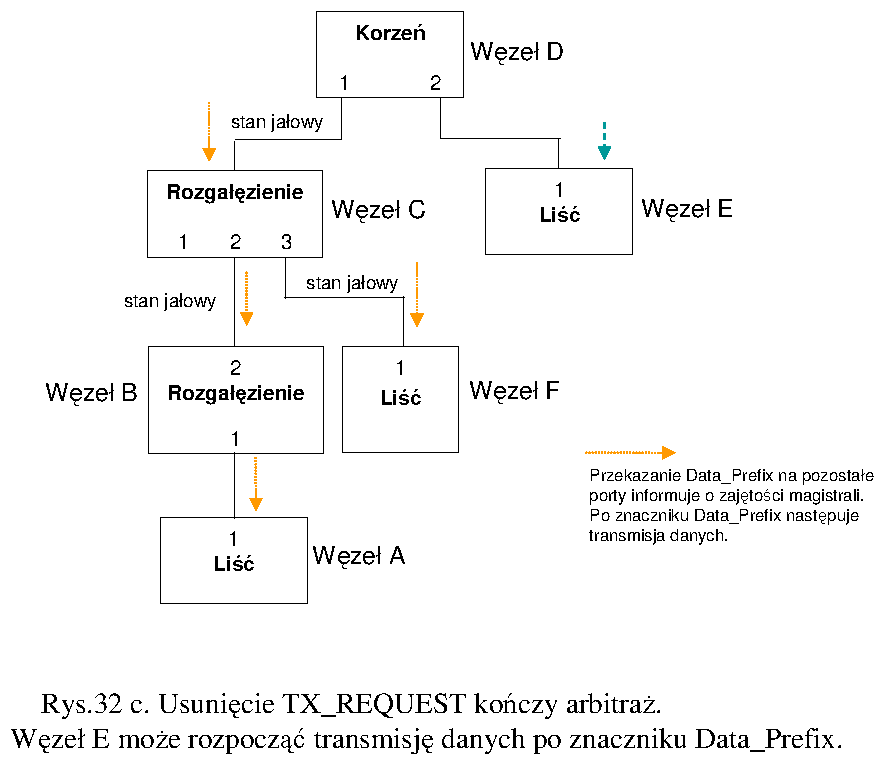
\includegraphics[width=9cm]{./wyklady/FIREWIRE_38_1.pdf}\\\\
\subsubsection{Arbitraż asynchroniczny}
\textbf{Zasada równych szans}
\begin{itemize}
	\item Węzły asynchroniczne do wykonania transakcji nie wymagają alokacji pasma.
	\item Działanie węzłów asynchronicznych polega na rotacyjnym przekazywaniu priorytetu (\emph{fairness interval} - „interwał równych szans”).
	\item Węzły asynchroniczne, które mają rozpoczęte transakcje uzyskują dostęp do magistrali w celu wykonania asynchronicznej subakcji (przesłania jednego pakietu).
	\item Kolejność przydziału zależy od położenia węzła w drzewie systemu. Węzły położone bliżej korzenia uzyskają dostęp przed węzłami bardziej oddalonymi.
	\item Łączny czas wykonania subakcji przez wszystkie węzły nazywa się \emph{fairness interval}.
	\item W tym czasie każdy węzeł uzyska dostęp do magistrali, aby wykonać subakcję.
	\item Dostęp do magistrali węzeł zarządzający przekazuje „rotacyjnie”.
	\item Następna subakcja będzie mogła być wykonana w kolejnym interwale równych szans.
\end{itemize}
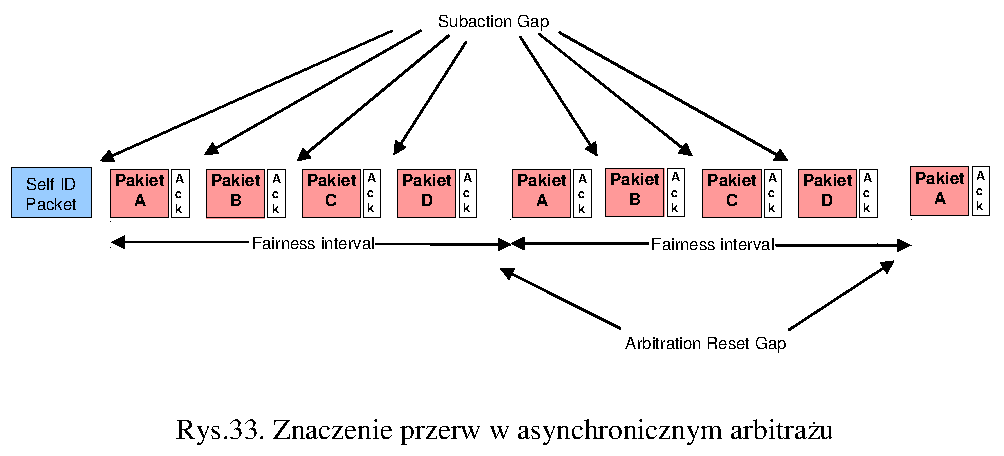
\includegraphics[width=9cm]{./wyklady/FIREWIRE_40_1.pdf}\\\\
\textbf{Odesłanie potwierdzenia, dostęp natychmiastowy}
\begin{itemize}
	\item Węzeł, który zainicjował asynchroniczną transakcję może sam być odbiorcą transakcji zainicjowanej przez inny węzeł.
	\item Warstwa połączeniowa węzła musi potwierdzić odbiór pakietu poprzez odesłanie potwierdzenia korzystając z usługi \emph{Immediate Arbitration Service} (\emph{IAS}) warstwy PHY.
	\item Warstwa PHY po otrzymaniu żądania usługi \emph{IAS} nie rywalizuje o dostęp do magistrali i bezpośrednio po wykryciu przerwy \emph{Acknowledge Gap} (0.04 do 0.05 $\mu{s}$) sygnalizuje warstwie LINK, że jest gotowa do przesłania pakietu potwierdzenia.
	\item Warstwa połączeniowa przekazuje pakiet potwierdzenia do portu za pośrednictwem warstwy PHY.
\end{itemize}
\subsubsection{Arbitraż izochroniczny}
\begin{itemize}
	\item Arbitraż izochroniczny rozpoczyna się natychmiast po rozgłoszeniu pakietu \emph{Cycle Start}, traktowanego jako znacznik początku cyklu.
	\item Po czasie 0.04 ms węzły izochroniczne pragnące uzyskać dostęp do magistrali rozpoczynają rywalizację o łącze.
	\item Węzeł, który wygra arbitraż wykonuje transakcję, po której magistrala powraca do stanu jałowego. Stan jałowy magistrali trwający przez 0.04 ms traktowany jest jako przerwa izochroniczna (\emph{Isochronous Gap}), po której rozpoczyna się arbitraż kolejnych węzłów izochronicznych zgłaszających żądanie transmisji.
	\item Przerwa izochroniczna trwa tyle samo, co \emph{Acknowledge Gap} dla transakcji asynchronicznych i jest znacznie mniejsza od \emph{Subaction Gap}. W ten sposób żaden węzeł asynchroniczny nie uzyska dostępu do magistrali zanim wszystkie węzły izochroniczne nie wykonają swoich transakcji.
	\item Cykl izochroniczny trwa 125 $\mu{s}$. Poszczególne węzły izochroniczne w ramach cyklu mają przydzielone pasmo (tzw. kanał), które jest częścią interwału 125 $\mu{s}$.
	\item Za przydział pasma odpowiedzialny jest węzeł zarządzający zasobami izochronicznymi. Jeżeli węzły izochroniczne nie wykorzystają pełnych 125 ms, w ramach wolnego czasu realizowane są transakcje asynchroniczne.
\end{itemize}
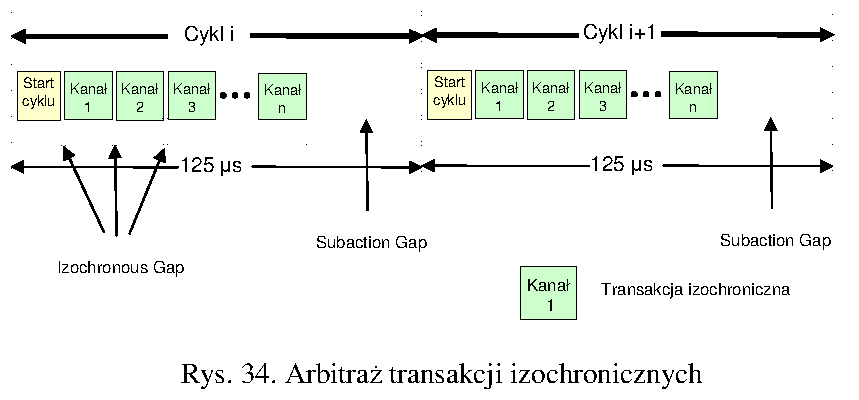
\includegraphics[width=9cm]{./wyklady/FIREWIRE_43_1.pdf}\\
Pakiet \emph{Cycle Start} generowany jest co 125 $\mu{s}$ przez węzeł będący korzeniem systemu.
\subsubsection{Łączenie arbitraży izochronicznego i asynchronicznego}
\begin{itemize}
	\item W ramach wolnego miejsca w interwale 125 $\mu{s}$ niewykorzystanego przez transakcje izochroniczne wykonywane są transakcje asynchroniczne.
	\item 80\% cyklu przydzielone jest transakcjom izochronicznym, a tylko 20\% transakcjom asynchronicznym.
	\item Transakcje izochroniczne wykonywane są w kolejnych 125 $\mu{s}$ cyklach (wartość nominalna), natomiast transakcje asynchroniczne w ramach interwału równych szans, którego długość zależy od liczby węzłów asynchronicznych jednocześnie żądających dostępu do łącza.
\end{itemize}
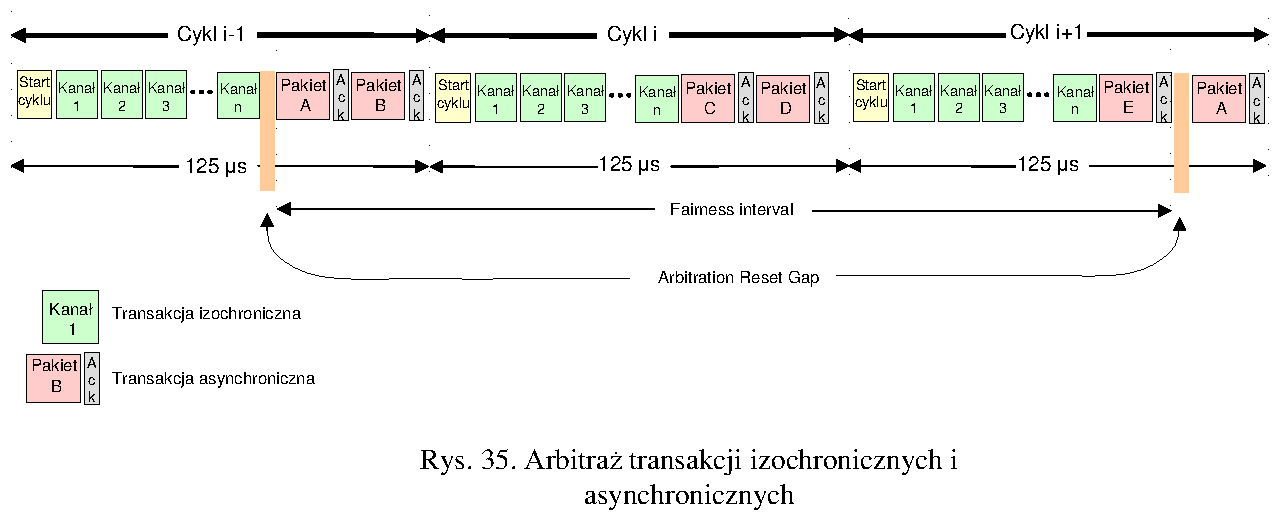
\includegraphics[width=9cm]{./wyklady/FIREWIRE_45_1.pdf}\\

\subsection{Pakiety}
\begin{itemize}
	\item \textbf{Pakiety izochroniczne} - Pakiety izochroniczne transmitowane są jako grupowe lub rozgłoszeniowe do jednego lub więcej węzłów.
	\item Transakcje izochroniczne:\\
	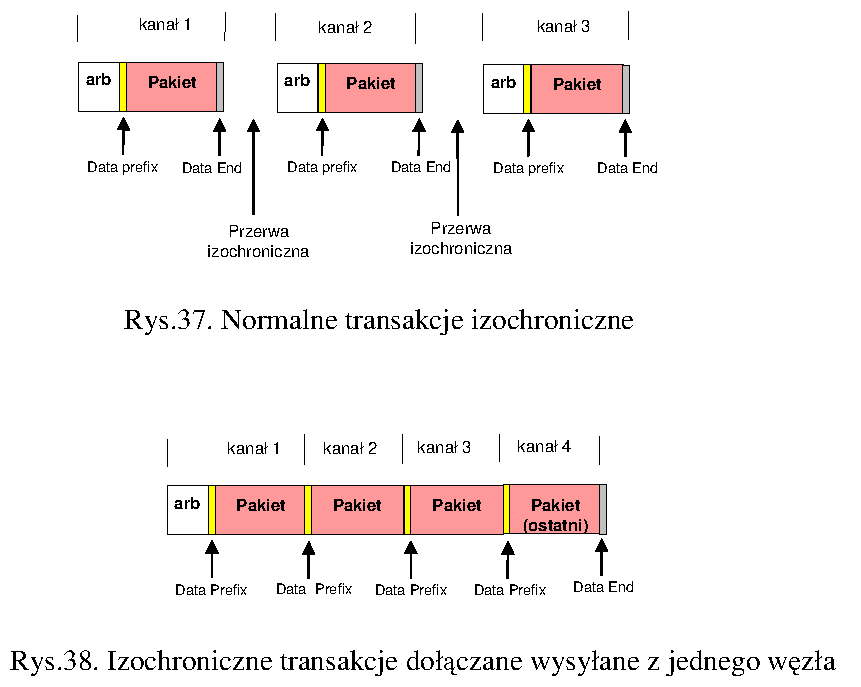
\includegraphics[width=7cm]{./wyklady/FIREWIRE_48_1.pdf}
	\item \textbf{Pakiety warstwy fizycznej}
	\begin{itemize}
		\item Standard IEEE 1394-1995 definiuje 3 pakiety PHY:
		\begin{itemize}
			\item Self Identyfication (Self-ID)
			\item Link-On
			\item PHY Configuration
		\end{itemize}
		\item Wersja 1394a rozszerza zestaw o pakiety:
		\begin{itemize}
			\item Ping
			\item Remote Access
			\item Remote Reply
			\item Remote Command
			\item Resume
		\end{itemize}
		\item Elementem procesu konfigurującego system IEEE-1394 do komunikacji jest nadanie każdemu węzłowi unikatowego identyfikatora oraz poinformowanie pozostałych węzłów ystemu o możliwościach transmisyjnych danego węzła.
		\item Te operacje wykonywane są za pomocą pakietów Self-ID rozgłaszanych przez węzły bezpośrednio po resecie i określeniu topologii systemu (identyfikacji drzewa).
	\end{itemize}
\end{itemize}

\subsection{Interfejs LINK-PHY}
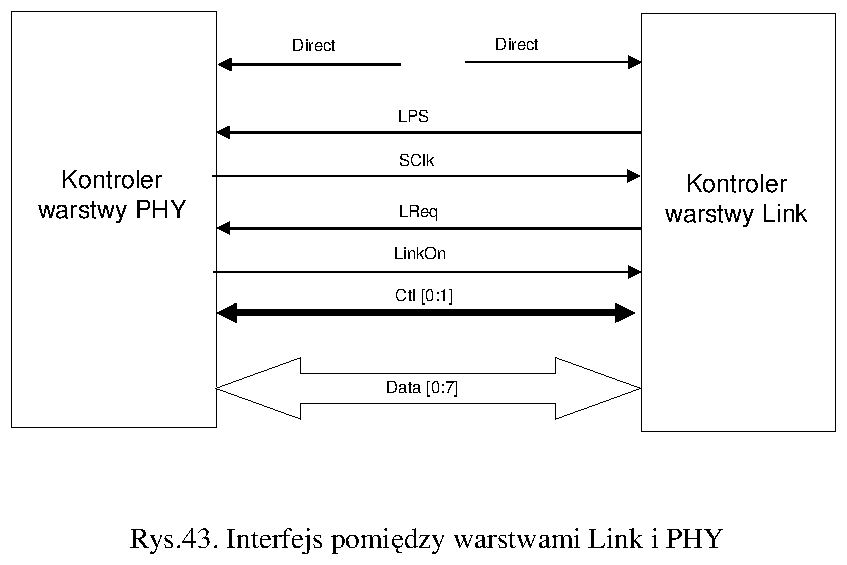
\includegraphics[width=7cm]{./wyklady/FIREWIRE_53_1.pdf}

\subsection{Ponowienie transakcji}
Wyróżniono dwa sposoby ponowienia transmisji pakietu:
\begin{itemize}
	\item jednofazowa repetycja (\emph{single phase retry}),
	\item dwufazowa repetycja (\emph{dual phase retry}).
\end{itemize}
Obsługa błędów jest zadaniem warstw transakcji lub aplikacji, przy czym obowiązują tu następujące zasady:
\begin{itemize}
	\item Reakcja na przekłamanie pakietu przez węzeł odbiorcy (przekłamanie pakietu przychodzącego)\\
	Błąd wykrywa warstwa liniowa węzła odbierającego pakiet i zawiadamia o tym warstwę transakcji.\\
	Warstwa transakcji nie przekazuje uszkodzonego pakietu do aplikacji, natomiast wysyła stosowne potwierdzenie negatywne do węzła będącego źródłem pakietu.
	\item Reakcja na powiadomienie o przekłamaniu pakietu przez węzeł nadawcy.\\
	Węzeł będący źródłem pakietu dowiaduje się o jego przekłamaniu po odebraniu potwierdzenia negatywnego.\\
	Warstwa aplikacji tego węzła jest odpowiedzialna za ewentualne powtórzenie transakcji.
\end{itemize}

\subsection{Konfiguracja magistrali}
\subsubsection{Reset magistrali}
\textbf{Przyczyny resetu}:
\begin{itemize}
	\item włączenie nowego urządzenia do systemu,
	\item odłączenie urządzenia,
	\item włączenie/wyłączenie zasilania urządzenia oraz błędy zasilania, jak np. jego chwilowe zaniki.\\
	(chodzi tu o zasilanie warstwy fizycznej węzła; włączenie/wyłączenie zasilania warstw połączeniowej i wyższych nie jest przyczyną resetu)
	\item inicjalizacja programowa, na żądanie aplikacji.
\end{itemize}
Reset jest „rozgłaszany” do wszystkich węzłów systemu.\\
Rezultatem Resetu jest:
\begin{itemize}
	\item Zwolnienie magistrali (przejście wszystkich segmentów do stanu jałowego);
	\item Inicjalizacja niektórych rejestrów warstwy PHY oraz pewnych pól w wybranych rejestrach warstwy PHY, co prowadzi do usunięcia wszystkich ustawień konfiguracyjnych portu (w szczególności identyfikatorów \emph{parent} lub \emph{child}, które informują o topologii systemu oraz identyfikatorów węzła);
	\item Inicjalizacja wybranych rejestrów CSR dokonywana przez warstwę LINK (LINK jest powiadamiana o resecie przez PHY).
\end{itemize}
\subsubsection{Identyfikacja drzewa systemu (Tree\_ID)}
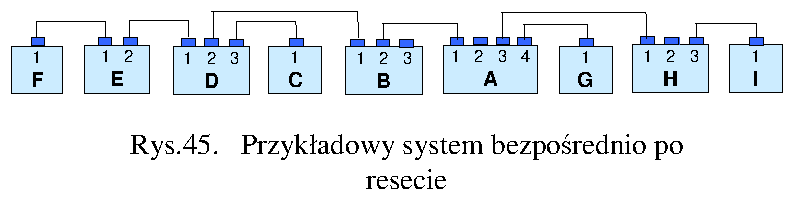
\includegraphics[width=7cm]{./wyklady/FIREWIRE_58_1.pdf}\\
Identyfikacja drzewa oparta jest na stanach interfejsu określanych przez połączone ze sobą porty, a wykrywanych przez komparatory arbitrażowe.\\
W procesie wykorzystywane są następujące stany interfejsu:
\begin{itemize}
	\item Parent\_Notify: STPA=0, STPB = Z, czyli 0Z
	\item Child\_Notify: STPA=1, STPB = Z, czyli 01
\end{itemize}
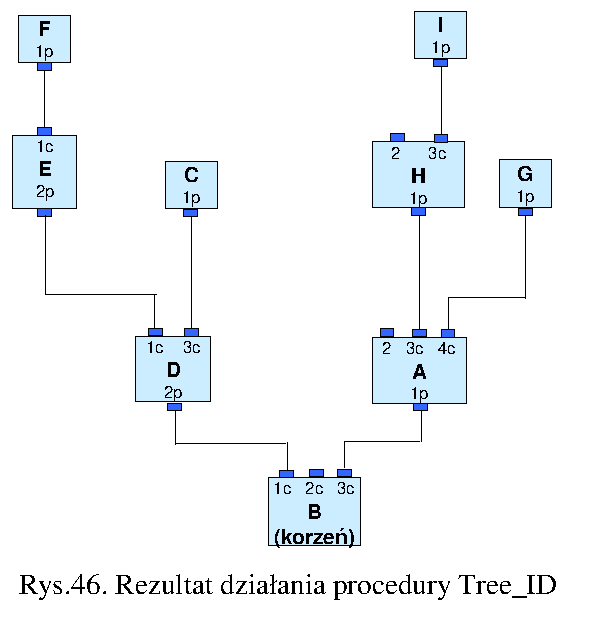
\includegraphics[width=7cm]{./wyklady/FIREWIRE_60_1.pdf}
\subsubsection{Samoidentyfikacja (Self\_ID)}
Samoidentyfikacja oparta jest na stanach interfejsu określanych przez połączone ze sobą porty, a wykrywanych przez komparatory arbitrażowe.\\
W procesie wykorzystywane są następujące stany interfejsu:
\begin{itemize}
	\item Self\_Id\_Grant (Arb\_Grant): STPA=Z, STPB =0, czyli Z0
	\item Data\_Prefix: STPA=0, STPB =1, czyli 01
	\item Identification\_Done: STPA=1, STPB =Z, czyli 1Z
\end{itemize}
\textbf{Rezultatem procedury Self\_Id jest}:
\begin{itemize}
	\item przypisanie każdemu węzłowi unikatowego identyfikatora pełniącego rolę adresu,
	\item rozesłanie pakietów self\_id z każdego portu do wszystkich pozostałych węzłów,
	które zawierają informacje o możliwościach i wymaganiach komunikacyjnych
	danego węzła,
	\item przypisanie każdemu portowi znacznika ID (zidentyfikowany) oznaczającego,
	że w segmencie magistrali, z którego korzysta dany port została określona
	szybkość transmisji.
\end{itemize}
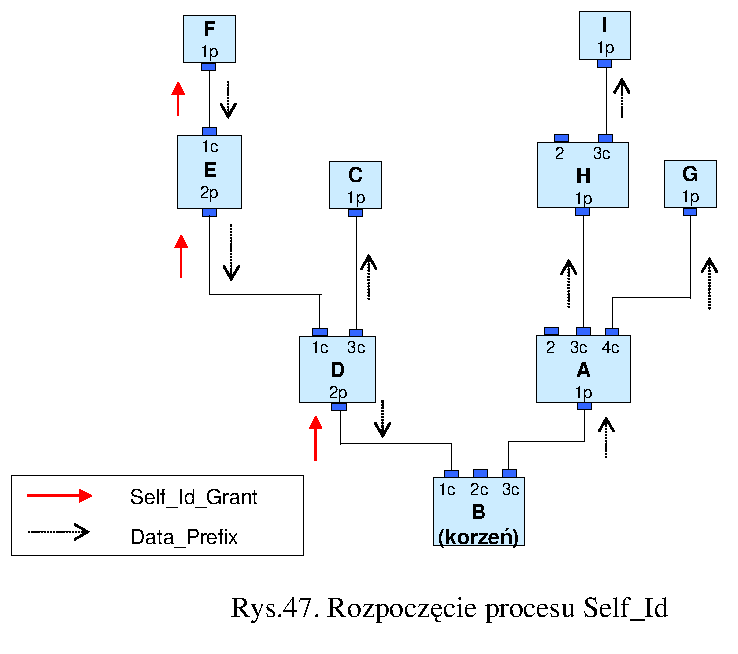
\includegraphics[width=7cm]{./wyklady/FIREWIRE_62_1.pdf}
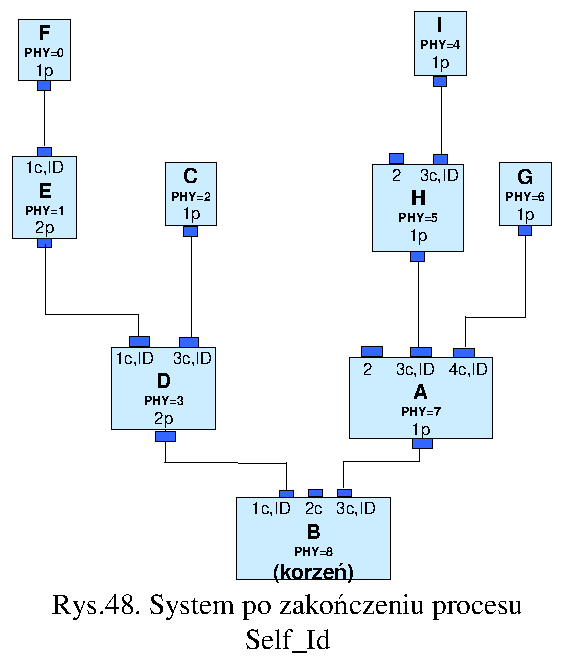
\includegraphics[width=7cm]{./wyklady/FIREWIRE_63_1.pdf}

\subsection{Zarządzanie zasilaniem}
\subsubsection{Najważniejsze cechy systemu zasilania}:
\begin{itemize}
	\item Urządzenia mogą posiadać zasilanie własne (lokalne) lub korzystać z zasilania systemowego. Możliwe jest udostępnianie zasilania (nieregulowane napięcie z zakresu 8 do 40 VDC) innym urządzeniom za	pośrednictwem magistrali systemowej. Część układów urządzenia może być zasilana ze źródła lokalnego, a inne wykorzystywać zasilanie systemowe.
	\item Zasilanie lokalne powinno być separowane za pośrednictwem diody od przewodów dystrybucji zasilania systemowego.
	\item Każde urządzenie musi informować o zapotrzebowaniu na zasilanie lub możliwości jego udostępnienia innym urządzeniom za pośrednictwem pakietu Self\_ID przekazywanego w procesie konfiguracji systemu.
	\item Bezpośrednio po resecie, urządzeniu wolno pobierać z zasilania systemowego do 1 W. Po zakończeniu konfiguracji systemu, kiedy wiadomo, jaka moc jest dostępna oraz jakie jest zapotrzebowanie urządzeń na zasilanie, możliwe jest przydzielenie urządzeniu większej mocy.\\
	Kalkulację mocy w systemie przeprowadza Zarządca magistrali. Pod nieobecność Zarządcy magistrali, Zarządca zasobów izochronicznych jest odpowiedzialny za rozesłanie pakietów Link\_ON włączających zasilanie w węzłach, które korzystają z zasilania systemowego.
	\item Do przekazywania zasilania służy 6 kontaktowe złącze z zaciskami VP i VG.
\end{itemize}
\subsubsection{W dokumencie Power Distribution wyróżniono}:
\begin{itemize}
	\item dostawcę zasilania (\emph{Power Provider})
	\item alternatywnego dostawcę zasilania (\emph{Alternate Power Provider})
	\item konsumenta zasilania (\emph{Power Consumer})
	\item węzeł z własnym źródłem zasilania
\end{itemize}
\subsubsection{Dostawca zasilania}
Dostawca zasilania udostępnia innym węzłom zasilanie pochodzące z własnego źródła wykorzystując do tego celu 6 kontaktowy konektor na każdym porcie.\\
Napięcie na zaciskach zasilania w portach dostawcy jest stałe i nieregulowane (zakres 22 do 33 V) oraz nie zależy od żadnych zdarzeń na magistrali sygnałowej.\\
Dostawcy zasilania deklarują klasę zasilania 1,2 lub 3 w zależności od mocy, którą są w stanie dostarczyć.\\
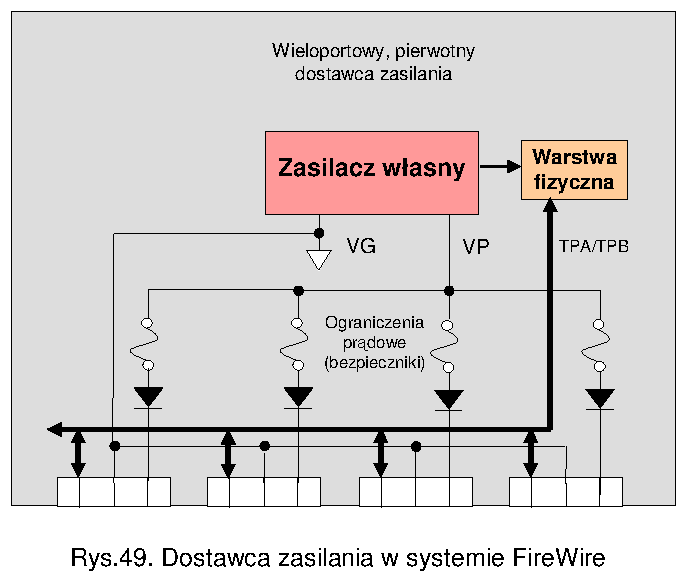
\includegraphics[width=7cm]{./wyklady/FIREWIRE_66_1.pdf}
\subsubsection{Alternatywny dostawca zasilania}
Dostawca alternatywny (DA) jest podklasą dostawcy zasilania.\\
DA dostarcza mniejszą moc od dostawcy pierwotnego, i obowiązują go mniejsze restrykcje.\\
DA ze złączy 6 kontaktowych.\\
Zaleca się żeby DA posiadał 2 porty.\\
W przypadku awarii zasilania własnego, dostawca alternatywny może korzystać z zasilania systemowego w celu podtrzymania funkcjonowania warstwy fizycznej i przekazywania ruchu pomiędzy portami.\\
W pakiecie Self\_ID dostawca alternatywny raportuje klasę zasilania 4\\
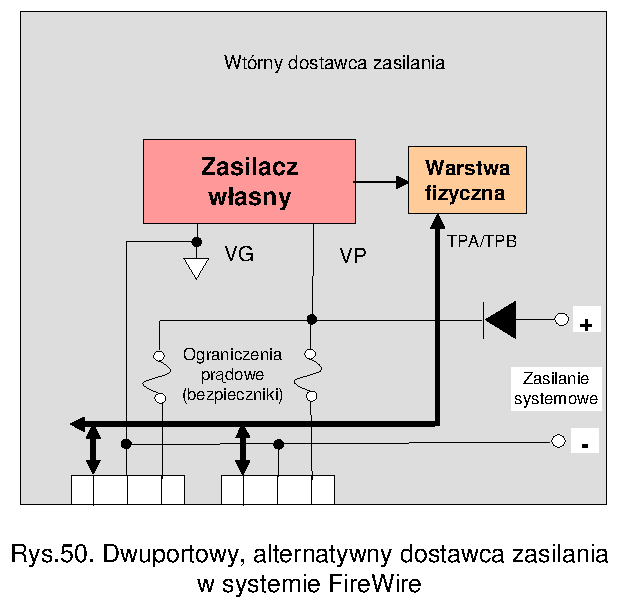
\includegraphics[width=7cm]{./wyklady/FIREWIRE_67_1.pdf}
\subsubsection{Konsument zasilania}
Konsument zasilania (KZ) wyposażony jest tylko w jeden port 6 kontaktowy, przez który pobiera prąd zasilania (pozostałe porty, o ile istnieją, muszą być 4 kontaktowe).\\
KZ raportuje w pakiecie Self\_ID klasę zasilania 4,6 lub 7.\\
Konsumenci zasilania mogą pobierać prąd zasilania z systemu lub zachowywać się „neutralnie”, tzn. wykorzystywać własne źródło zasilania nie udostępniając go innym urządzeniom.\\
Od konsumenta, który korzysta z własnego źródła zasilania wymaga się, aby przekazywał zasilanie systemowe pomiędzy swoimi portami, a w przypadku węzłów wieloportowych, wymaga się również obecności ograniczenia prądowego na każdym porcie. Przekazywanie zasilania pomiędzy portami musi być blokowane, gdy węzeł ma wyłączone zasilanie warstwy fizycznej.\\
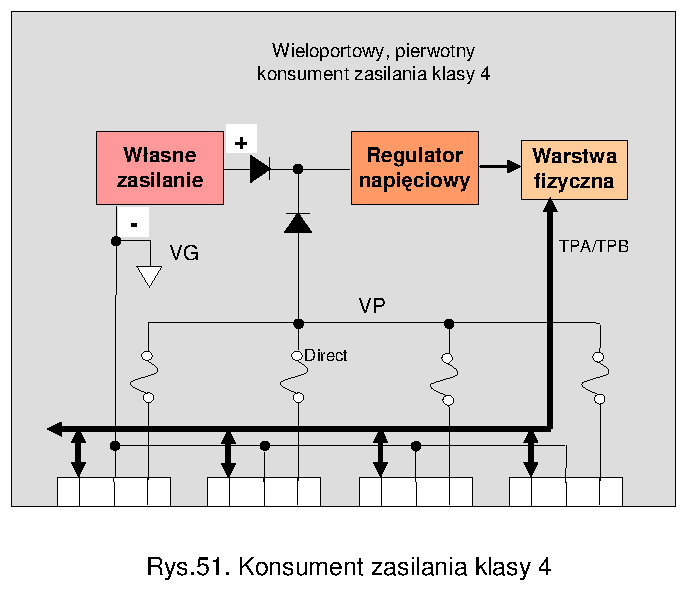
\includegraphics[width=7cm]{./wyklady/FIREWIRE_68_1.pdf}\\\\
Najprostszym konsumentem zasilania jest węzeł, którego warstwa fizyczna zasilana jest bezpośrednio z magistrali.\\
Układy wykonujące funkcje wyższych warstw protokołowych korzystają na ogół z zasilania własnego.\\
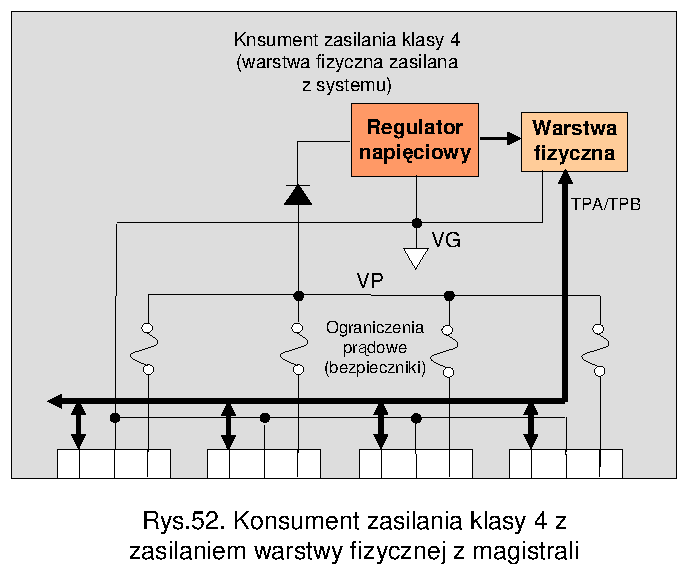
\includegraphics[width=7cm]{./wyklady/FIREWIRE_69_1.pdf}
\subsubsection{Zawieszenie portu}
Zawieszenie portu (\emph{port suspend}) powoduje blokadę ruchu w porcie, a w konsekwencji również blokadę ruchu w całej gałęzi (domenie urządzeń) obsługiwanej przez ten port.\\
Zawieszone urządzenie wymaga tylko nieznacznej mocy do podtrzymania swojej konfiguracji. Ze stanu zawieszenia można powrócić do normalnej aktywności realizując tzw. wznowienie (\emph{resume}).\\
Sposoby zawieszenia portu:
\begin{itemize}
	\item stosownym rozkazem zdalnym lub lokalnym,
	\item poprzez detekcję stanu RX\_SUSPEND interfejsu,
	\item w konsekwencji wykrycia stanu RX\_SUSPEND na innym porcie tego samego węzła,
	\item poprzez detekcję stanu RX\_DISABLE\_NOTIFY interfejsu.
\end{itemize}
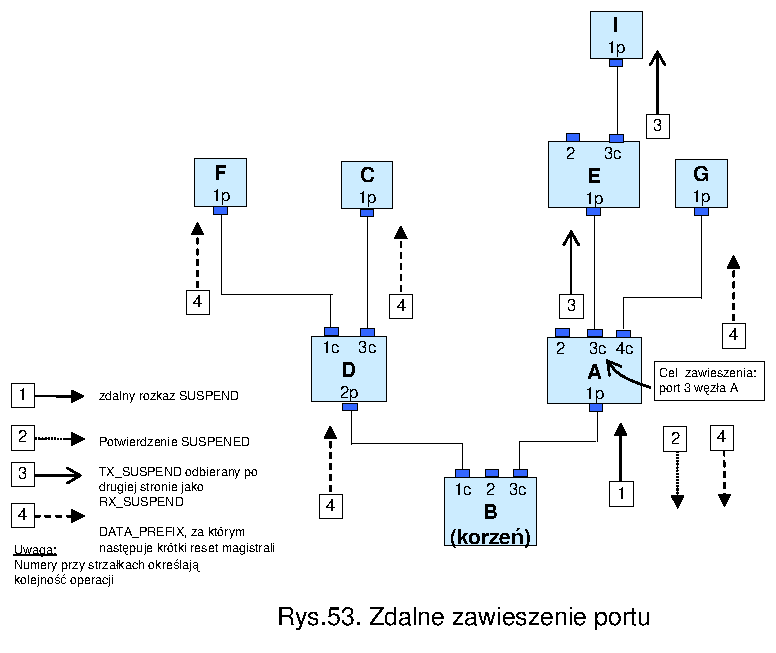
\includegraphics[width=7cm]{./wyklady/FIREWIRE_70_1.pdf}
\subsubsection{Wznowienie}
Wznowienie (\emph{Resume}) jest powrotem portu do normalnego działania po uprzednim zawieszeniu.\\
Wyróżniono 3 sposoby wznowienia:
\begin{itemize}
	\item globalne, realizowane poprzez rozgłoszenie pakietu wznowienia do wszystkich węzłów
	\item selektywne, realizowane za pomocą zdalnego pakietu PHY, kierowane do konkretnego, zablokowanego lub zawieszonego portu
	\item z inicjatywy węzła, w którym znajduje się zawieszony port, po wystąpieniu zdarzenia, którego obsługa wymaga przywrócenia komunikacji na zawieszonym porcie
\end{itemize}

